\RCS$Revision: 230053 $
\RCS$HeadURL: svn+ssh://svn.cern.ch/reps/tdr2/notes/AN-14-062/trunk/AN-14-062.tex $
\RCS$Id: AN-14-062.tex 230053 2014-03-05 06:58:25Z syu $
%%%%%%%%%%%%% local definitions %%%%%%%%%%%%%%%%%%%%%
% This allows for switching between one column and two column (cms@external) layouts
% The widths should  be modified for your particular figures. You'll need additional copies if you have more than one standard figure size.
\newlength\cmsFigWidth
\ifthenelse{\boolean{cms@external}}{\setlength\cmsFigWidth{0.85\columnwidth}}{\setlength\cmsFigWidth{0.4\textwidth}}
\ifthenelse{\boolean{cms@external}}{\providecommand{\cmsLeft}{top}}{\providecommand{\cmsLeft}{left}}
\ifthenelse{\boolean{cms@external}}{\providecommand{\cmsRight}{bottom}}{\providecommand{\cmsRight}{right}}
%%%%%%%%%%%%%%%  Title page %%%%%%%%%%%%%%%%%%%%%%%%
\cmsNoteHeader{MOST 103-2112-M-008-010-MY3} % This is over-written in the CMS environment: useful as preprint no. for export versions
\newcommand{\Xtohh}{\ensuremath{\X\to\Ph\Ph}\xspace}

\newcommand{\qqbarpr}{\ensuremath{\Pq\Paq^({}'^){}}\xspace}
\newcommand{\lnujet}{\ensuremath{\ell \nu}+jet\xspace}
\newcommand{\lljet}{\ensuremath{\ell \ell}+jet\xspace}
\newcommand{\PV}{\ensuremath{\mathrm{V}}}
\newcommand{\nsubj}{\ensuremath{\tau_{21}}}%
\newcommand{\Vo}{\ensuremath{\mathrm{V}}\xspace}%
\newcommand{\mVV}{\ensuremath{m_{\Vo\Vo}}\xspace}%
\newcommand{\Grav}{\ensuremath{\PXXG_{\mathrm{bulk}}}}%
\newcommand{\ktilde}{\ensuremath{k/\overline{M}_\mathrm{Pl}}\xspace}%
\newcommand{\pb}{\ensuremath{\cmsSymbolFace{pb}}\xspace}
\newcommand{\X}{\ensuremath{\cmsSymbolFace{X}}\xspace}
\newcommand{\A}{\ensuremath{\cmsSymbolFace{A}}\xspace}
\newcommand{\V}{\ensuremath{\cmsSymbolFace{V}}\xspace}
\newcommand{\h}{\ensuremath{\cmsSymbolFace{h}}\xspace}
\renewcommand{\PW}{\ensuremath{\cmsSymbolFace{W}}\xspace}
\newcommand{\XtoVh}{\ensuremath{\X\to\V\Ph}\xspace}
\newcommand{\XtoZh}{\ensuremath{\X\to\Z\Ph}\xspace}
\newcommand{\XtoWh}{\ensuremath{\X\to\PW\Ph}\xspace}
\newcommand{\AtoZh}{\ensuremath{\A\to\Z\Ph}\xspace}
\newcommand{\htobb}{\ensuremath{\Ph\to\bbbar}\xspace}
\newcommand{\Ztoll}{\ensuremath{\Z\to\ell\ell}\xspace}
\newcommand{\Ztoee}{\ensuremath{\Z\to\Pe\Pe}\xspace}
\newcommand{\Ztomm}{\ensuremath{\Z\to\mu\mu}\xspace}
\newcommand{\Ztonn}{\ensuremath{\Z\to\nu\nu}\xspace}
\newcommand{\Atollbb}{\ensuremath{\A\to\Z\Ph\to{\ell\ell}\bbbar}\xspace}
\newcommand{\Xtollbb}{\ensuremath{\X\to\Z\Ph\to{\ell\ell}\bbbar}\xspace}
\newcommand{\Xtoeebb}{\ensuremath{\X\to\Z\Ph\to{\Pe\Pe}\bbbar}\xspace}
\newcommand{\Xtommbb}{\ensuremath{\X\to\Z\Ph\to{\mu\mu}\bbbar}\xspace}
\newcommand{\Xtolnbb}{\ensuremath{\X\to\PW\Ph\to{\ell\nu}\bbbar}\xspace}
\newcommand{\Xtoenbb}{\ensuremath{\X\to\PW\Ph\to{\Pe\nu}\bbbar}\xspace}
\newcommand{\Xtomnbb}{\ensuremath{\X\to\PW\Ph\to{\mu\nu}\bbbar}\xspace}
\newcommand{\Xtonnbb}{\ensuremath{\X\to\Z\Ph\to{\nu\nu}\bbbar}\xspace}
\renewcommand{\PHpm}{\ensuremath{\PH^\pm}\xspace}
\newcommand{\Zh}{\ensuremath{\Z\Ph}\xspace}
\newcommand{\Wh}{\ensuremath{\PW\Ph}\xspace}
\newcommand{\VH}{\ensuremath{\V\Ph}\xspace}
\newcommand{\VV}{\ensuremath{\V\V}\xspace}
\newcommand{\ST}{\ensuremath{\text{ST}}\xspace}
\newcommand{\Vjets}{\ensuremath{\V\text{+jets}}\xspace}
\newcommand{\mVH}{\ensuremath{m_{\VH}}\xspace}
\newcommand{\mX}{\ensuremath{m_{\X}}\xspace}
\newcommand{\mT}{\ensuremath{m_{\text{T}}}\xspace}
\newcommand{\mA}{\ensuremath{m_{\A}}\xspace}
\newcommand{\mh}{\ensuremath{m_{\Ph}}\xspace}
\newcommand{\mHpm}{\ensuremath{m_{\PHpm}}\xspace}
\newcommand{\mt}{\ensuremath{m_{\PQt}}\xspace}
\newcommand{\mtX}{\ensuremath{m_{\PQt}^{\X}}\xspace}
\newcommand{\ttbarV}{\ensuremath{\ttbar V\xspace}}
\newcommand{\mbb}{\ensuremath{m_{\PQb\PQb}}\xspace}
\newcommand{\mll}{\ensuremath{m_{\ell\ell}}\xspace}
\newcommand{\mllbb}{\ensuremath{m_{\ell\ell\PQb\PQb}}\xspace}
\newcommand{\mlnbb}{\ensuremath{m_{\ell\nu\PQb\PQb}}\xspace}
\newcommand{\mTnnbb}{\ensuremath{m^T_{\nu\nu\PQb\PQb}}\xspace}
\newcommand{\cosba}{\ensuremath{\cos(\beta-\alpha)}\xspace}
\newcommand{\B}{\ensuremath{\mathcal{B}}}
\newcommand{\fb}{\ensuremath{\,\text{fb}}\xspace}
\newcommand{\Zb}{\ensuremath{\Z+\PQb}\xspace}
\newcommand{\Zbbbar}{\ensuremath{\Z+\bbbar}\xspace}
%\newcommand{\qqbar}{\ensuremath{\cPq\cPaq}\xspace}
\newcommand{\MHT}{\ensuremath{H_\text{T}^\text{miss}}\xspace}

\renewcommand{\HGG}{\ensuremath{\Ph\rightarrow\gamma\gamma}\xspace}
\newcommand{\Hbb}{\ensuremath{\Ph\rightarrow\PQb\PAQb}\xspace}
\newcommand{\mzp}{\ensuremath{m_{\PZpr}}\xspace}
\renewcommand{\Az}{\ensuremath{\cmsSymbolFace{A}}\xspace}
\newcommand{\ptm}{\ensuremath{p_{\mathrm{T}}^{\text{miss}}}\xspace}
\renewcommand{\MET}{\ptm}
\renewcommand{\ETm}{\ptm}
\newcommand{\maz}{\ensuremath{m_{\Az}}\xspace}
\newcommand{\mdm}{\ensuremath{m_{\chi}}\xspace}
\newcommand{\gzp}{\ensuremath{g_{\PZpr}}\xspace}
\newcommand{\MADGRAPHAMC} {\MADGRAPH{}5\_a\MCATNLO}
\newcommand{\x}{\ensuremath{\phantom{0}}}

\providecommand{\Ph}{\ensuremath{\cmsSymbolFace{h}}\xspace}
\providecommand{\PQb}{\cPqb}
\providecommand{\PQt}{\cPqt}
\providecommand{\PZ}{\ensuremath{\cmsSymbolFace{Z}}\xspace}
\providecommand{\PW}{\ensuremath{\cmsSymbolFace{W}}\xspace}
\newcommand{\ttjets}{\ensuremath{\cPqt\overline{\cPqt}}+jets\xspace}
\newcommand{\wjets}{\PW+jets\xspace}
\newcommand{\bjet}{\cPqb~jet\xspace}
\newcommand{\bjets}{\cPqb~jets\xspace}
\newcommand{\sm}{the standard model\xspace}
\newcommand{\mc}{Monte Carlo\xspace}
\newcommand{\com}{13\TeV\xspace}
\newcommand{\intLumi}{35.9\fbinv}

\newcommand{\Hbbt}{double-\cPqb\,tagger\xspace}
\newcommand{\Sjbt}{subjet \PQb\,tagger\xspace}
\newcommand{\GRS}{\ensuremath{\mathrm{G}_\mathrm{RS}}\xspace}
\newcommand{\mjj}{\ensuremath{m_{\text{jj}}}\xspace}
\newcommand{\mjjs}{\ensuremath{m_{\text{jj}}^{\text{red}}}\xspace}
\newcommand{\Mjjs}{\ensuremath{m_{\text{jj}}^{\text{red}}}\xspace}
\newcommand{\mjjred}{\ensuremath{m_{\text{jj}}^{\text{red}}}\xspace}
\newcommand{\Mjjred}{\ensuremath{m_{\text{jj}}^{\text{red}}}\xspace}
\newcommand{\mH}{\ensuremath{m_{\text{\PH}}}\xspace}
\newcommand{\mx}{\ensuremath{m_{\text{X}}}\xspace}
\newcommand{\mux}{\ensuremath{\mu_{\text{X}}^{\text{CB}}}\xspace}
\newcommand{\nsub}{\ensuremath{\tau_{21}}\xspace}
\newcommand{\etaj}{\ensuremath{|\eta|}\xspace}
\newcommand{\deta}{\ensuremath{|\Delta\eta_{\text{jj}}|}\xspace}
\newcommand{\mjp}{\ensuremath{m_{\text{jet}}^{\text{pruned}}}\xspace}
\newcommand{\mjsd}{\ensuremath{m_{\text{jet}}^{\text{softdrop,puppi}}}\xspace}
\newcommand{\mj}{\ensuremath{m_{\text{jet}}}\xspace}
\newcommand{\mjone}{\ensuremath{m_{\text{j}_{1}}}\xspace}
\newcommand{\mjtwo}{\ensuremath{m_{\text{j}_{2}}}\xspace}
\newcommand{\LambdaR}{\ensuremath{\Lambda_{\text{R}}}\xspace}
\newcommand{\DeltaEta}{\ensuremath{\Delta\eta(\text{j}_{1}, \text{j}_{2})}\xspace}
\newcommand{\HH}{\PH\PH}
\newcommand{\sgx}{\ensuremath{\sigma_{\text{X}}^{\text{gaus}}}\xspace}
\newcommand{\scbx}{\ensuremath{\sigma_{\text{X}}^{\text{CB}}}\xspace}
\newcommand{\HbbHbb}{\ensuremath{\mathrm{\Hbb\Hbb}}\xspace} 
\newcommand{\XHbbHbb}{\ensuremath{\mathrm{X}\rightarrow\PH\PH\rightarrow\bbbar\bbbar}\xspace}




% >> Title: please make sure that the non-TeX equivalent is in PDFTitle below
\title{Travel Report (2017/06/19--2017/08/25): \bf{MOST 103-2112-M-008-010-MY3}}

% >> Authors
%Author is always "The CMS Collaboration" for PAS and papers, so author, etc, below will be ignored in those cases
%For multiple affiliations, create an address entry for the combination
%To mark authors as primary, use the \author* form
\address[NCU]{National Central University,  Chung-Li, Taiwan}
\author[NCU]{Shin-Shan Yu}


% >> Date
% The date is in yyyy/mm/dd format. Today has been
% redefined to match, but if the date needs to be fixed, please write it in this fashion.
% For papers and PAS, \today is taken as the date the head file (this one) was last modified according to svn: see the RCS Id string above.
% For the final version it is best to "touch" the head file to make sure it has the latest date.

% >> Abstract
% Abstract processing:
% 1. **DO NOT use \include or \input** to include the abstract: our abstract extractor will not search through other files than this one.
% 2. **DO NOT use %**                  to comment out sections of the abstract: the extractor will still grab those lines (and they won't be comments any longer!).
% 3. For PASs: **DO NOT use tex macros**         in the abstract: CDS MathJax processor used on the abstract doesn't understand them _and_ will only look within $$. The abstracts for papers are hand formatted so macros are okay.
\abstract{
This MOST travel report describes the research results during the trip of Prof. Shin-Shan Yu to CERN from 19 June 2017 to 25 August 2017. The results include finishing the 2015 mono-Higgs paper, preparing for the pre-approval/approval of the 2016 mono-Higgs analysis, synchronization of the mono-Higgs signal cross sections with ATLAS, implementation of the jet substructure study for the 100-\TeV colliders, preparing for the analysis of 2017 data, and analysis of the HGC test beam.
}


% >> PDF Metadata
% Do not comment out the following hypersetup lines (metadata). They will disappear in NODRAFT mode and are needed by CDS.
% Also: make sure that the values of the metadata items are sensible and are in plain text:
% (1) no TeX! -- for \sqrt{s} use sqrt(s) -- this will show with extra quote marks in the draft version but is okay).
% (2) no %.
% (3) No curly braces {}.
\hypersetup{%
pdfauthor={Shin-Shan Yu},%
pdftitle={Travel Report},%
pdfsubject={CMS},%
pdfkeywords={LHC, CMS, high-mass new particle, beyond the standard model, dark matter, phase 2 detector upgrade, boosted Higgs boson, di-boson}
}

\maketitle %maketitle comes after all the front information has been
\tableofcontents

%\tableofcontents
%%%%%%%%%%%%%%%%%%%%%%%%%%%%%%%%%%%%%%%%%%%%%%%%%%%%%%%%%%%%%%%%%%%%%%%%%%%%%%%
\section{Introduction}
My research activity during my CERN trip between 19 June to 25 August 2017 includes the following:
\begin{itemize}
 \item Addressing the comments from the JHEP referees on the 2015 mono-Higgs paper
 \item Serving the Analysis Review Committee (ARC) for the CMS analyses SMP-14-021, EXO-16-030, and B2G-17-013
 \item Synchronizing the cross sections of the baryonic Z’ and 2HDM+a models with the ATLAS mono-Higgs group
 \item Working with my postdoc Dr. Raman Khurana and the postdocs from MIT/Fermilab for the pre-approval/approval of the 2016 mono-Higgs results
 \item Working with and supervising my undergraduate student on the searches for DM mediators via their visible decays
 \item Analysis of the July 2017 HGC test beam data
 \item Implementing the analysis ntuple framework and prepare for 2017 data taking
 \item Testing and preparing the code to compute jet substructure variables using calo hits for the 100-TeV collider
\end{itemize}

I will describe in more detail for some of the items above.

%%%%%%%%%%%%%%%%%%%%%%%%%%%%%%%%%%%%%%%%%%%%%%%%%%%%%%%%%%%%%%%%%%%%%%%%%%%%%%%
\section{Addressing the comments from the JHEP referees on the 2015 mono-Higgs paper}
We received about 60 comments from the JHEP referees. I was in charge of addressing the comments related to the benchmark model we used. Particularly the following comments:
\begin{enumerate}
\item Finally, see also comments on the results below, the title of this paper contains the appealing term dark matter, but then the whole paper shows only results for one value of mchi, namely 100 GeV. The sentence before last should qualify clearly over which range of values of mchi (presumably between 0 and mA/2 - XX GeV) the limits quoted are valid. Also, the sentence should clearly state the other assumptions underlying the quoted limits, namely that tanbeta = 1 and gchi = 1.

{\bf Ans:} The choices we made, such as setting the DM mass to 100~\GeV, \gzp=0.8, $\tan\beta$ follow the recommendations of the ATLAS-CMS DM forum 
paper~\cite{Abercrombie:2015wmb}. However, these choices were decided in a rush, without a reason motivated by physics. Therefore, we had to trace back 
the reason using the current knowledge we had about the Z'-2HDM model. I did several studies and found out the formulas that describe the 
relationship between cross sections, ${\cal B}(\cPZpr\rightarrow \Az \Ph)$, and ${\cal B}(\Az\rightarrow\chi\bar{\chi})$, and the DM mass, \gzp, and 
$\tan\beta$ from Ref.~\cite{2HDM}. 

Regarding the fixed choice of \mdm, we have followed the recommendation of the ATLAS-CMS Dark Matter Forum paper: 1507.00966: fixing $\mdm = 100~\GeV$ and scanning the limits in the \maz - \mzp 2D plane. This choice has also been adopted by both the Run-I ATLAS paper Phys. Rev. D 93, 072007 (1510.06218) and the Run-II ATLAS paper using 2015 data Phys. Lett. B 765 (2016) 11 (1609.04572). 
In addition one should note that the branching fraction ${\cal B}(\Az\rightarrow \chi\bar{\chi})$ decreases as \mdm\ increases; therefore, the 
limits are also valid for $\mdm < 100~\GeV$.

In this model, since the DM pair are produced as a result of the decay of \Az, as long as \Az\ is produced on-shell and $\mdm<\maz/2$, the 
kinematic distributions have little dependence on \mdm. If one wants to produce limits as a function of \mdm, the limits could be scaled easily using the dependence of ${\cal B}(\Az\rightarrow \chi \chi)$ on \mdm as follows: 
\begin{tiny}
\begin{verbatim}
float gamma_chichi = (gdm*gdm*pow(ma0,2)*sqrt(pow(ma0,4)-4*pow(ma0*mchi,2)))/8.0/TMath::Pi()/pow(ma0,3); ## width of A0-> chi chi 

float gamma_tt = (3./pow(tb1,2)*pow(ma0*yt,2)*sqrt(pow(ma0,4)-4*pow(ma0*ymt,2)))/16.0/TMath::Pi()/pow(ma0,3); ## width of A0->tt 

float gamma_bb = (3.*pow(tb1,2)*pow(ma0*yb,2)*sqrt(pow(ma0,4)-4*pow(ma0*ymb,2)))/16.0/TMath::Pi()/pow(ma0,3); ## width of A0->bb 

float br = gamma_chichi/(gamma_tt1+gamma_bb1+gamma_chichi); 
\end{verbatim}
\end{tiny}
Considering $\tan\beta=1$, when $\maz=300~\GeV$, since $\Az\rightarrow \chi \chi$ is the dominant decay channel and the branching ratio is close to 
100\%, the variation of cross section is tiny; for example, for $\maz=300~\GeV$, the variation of cross section from $\mdm=0$ to $\mdm=140~\GeV$ is 
about 0.5\%. For larger \maz where 
$\Az\rightarrow \PQt\PAQt$ is also allowed, ${\cal B}(\Az\rightarrow\chi\chi)$ starts to have larger dependence on \mdm; for example, for 
$\maz=500~\GeV$, the variation of cross section from $\mdm=0$ to $\mdm=150~\GeV$ is about 10\%. 
See Fig.~\ref{fig:brmdm} for an example of ${\cal B}(\Az\rightarrow\chi\chi)$ vs \mdm\ for $\maz=300~\GeV$ and for $\maz=500~\GeV$. 

From the formula above, one could also see that the slope of ${\cal B}(\Az\rightarrow\chi\chi)$  v.s. \mdm\ increases as \mdm\ increases. Overall, 
for all the values of \maz\ we considered (300-800~\GeV), the variation of cross section from $\mdm=0$ to $\mdm=100~\GeV$ is within 7\% for 
$\tan\beta=1$. (For larger $\tan\beta$, the variation is even smaller. For $\tan\beta\approx0.3$, the variation is about 10\%.) However, as $\mdm$ 
approaches $\maz/2$, higher values of $\mdm$ simply reduce the ${\cal B}(\Az\rightarrow\chi\chi)$ and the effective cross sections significantly, 
and are beyond the sensitivity of this analysis. 
Because of this, the value of $\mdm=100~\GeV$ was recommended in the ATLAS-CMS forum paper arXiv:1507.00966.


\begin{figure}[htbp]
\centering
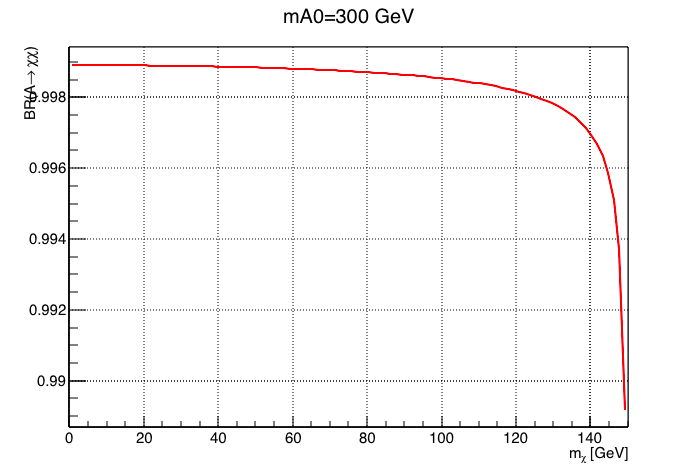
\includegraphics[width=0.45\textwidth]{brvsmchi_ma300.png}
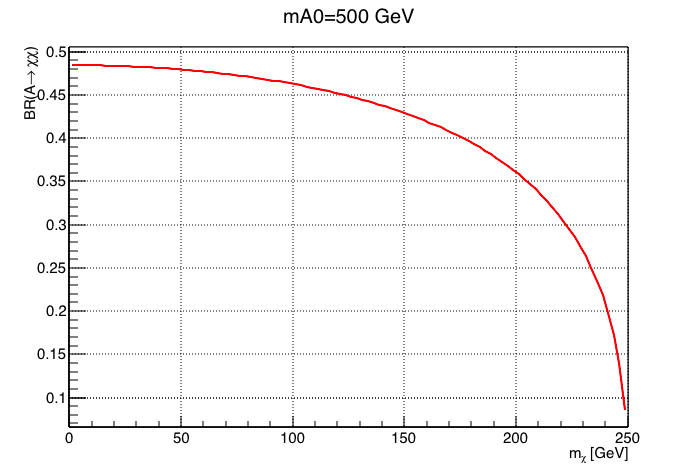
\includegraphics[width=0.45\textwidth]{brvsmchi_ma500.png}
\caption{The branching fraction ${\cal B}(\Az\rightarrow\chi\chi)$ as a function of \mdm, for $\maz=300~\GeV$ (left) and $\maz=500~\GeV$ (right), respectively. \label{fig:brmdm}}
\end{figure}



\item Concerning the above comment, I read reference 7 and one sees there that for values of tanbeta larger than unity the h to bb sensitivity disappears while the h to gg one does not. Given the importance given in this paper to the h to gg component of the search, why are larger values of tanbeta not explored to interpret the results?

{\bf Ans:} Indeed \HGG has better sensitivity than \Hbb at large $\tan\beta$, 
but only when the amount of data collected is huge enough, such as 300\fbinv. 
Note, for the range of \maz and \mzp we considered, the mass point 
$\maz=300~\GeV$ and $\mzp=600~\GeV$ has the largest cross section. 
When $\maz=300~\GeV$, $\tan\beta=1$ gives the largest cross section; coming 
from the combination of ${\cal B}(\cPZpr\rightarrow \Az\Ph)$ that scales with 
$\tan\beta^2/\sec\beta^4$ and ${\cal B}(\Az\rightarrow\chi\chi)$. See the 
dependence of cross section on $\tan\beta$ in Fig.~\ref{fig:brtanb}.
The expected number of signal events for \HGG is already less than 1 event 
for this mass point and $\tan\beta=1$. Therefore, we choose to focus on 
$\tan\beta=1$ in this first mono-Higgs paper at CMS. 

\begin{figure}[htbp]
\centering
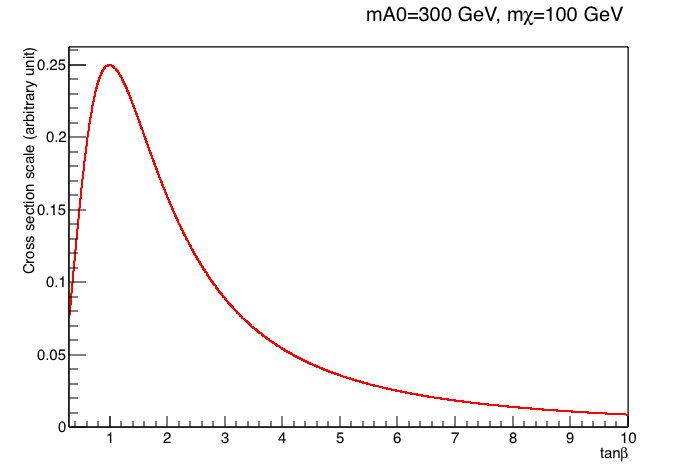
\includegraphics[width=0.7\textwidth]{tanb_ma300.png}
\caption{The mono-h cross section as a function of $\tan\beta$, 
for $\maz=300~\GeV$ and $\mdm=100~\GeV$. \label{fig:brtanb}}
\end{figure}



\item One other thing which puzzles me is what is the value of BR(Z* to Ah) with respect to BR(Z* to Zh) which surely may be sizable. Is this fixed by the choice of gZ* = 0.8 or the other choice of gZ* quoted later? Or does the choice of gZ* simply define the coupling of the Z* to quarks for its production cross section? I apologize for the perhaps confused set of questions, but I did really try to learn about these models when reading this paper and did not quite understand all the underlying assumptions from reading it.

{\bf Ans:} As you could see from Equations 16 and 17 of Ref.~\cite{2HDM}, \gzp 
cancels in the ratio of the decay widths of $\cPZpr\rightarrow \Az \Ph$ and 
$\cPZpr\rightarrow \cPZ\Ph$. The relative value of these two branching ratios 
is driven by $\tan\beta$ and \mzp, as indicated in Figure 6 of Ref.~\cite{2HDM}
 as well. Therefore, our choice of gz does not affect this relative 
contribution. In this first mono-Higgs paper, we do not consider the 
contribution of $\cPZpr\rightarrow\cPZ\Ph$, similar to what is done in the 
ATLAS run II paper. We have added a statement about this near the end of 
Section 1:

{\it “Note this analysis does not consider the contribution of another decay that gives similar mono-h signature,  $\cPZpr\rightarrow\cPZ\Ph$ where $\cPZ\rightarrow \nu\bar{\nu}$”} 
 

\item Just out of curiosity, I wonder where in ref 7 one can find this explicit equation? There is a related equation and a figure, but I could not derive it so easily, this is just a comment for my education, thanks. A few words justifying here why gZ* is 0.8 would be great for the non-expert reader.

{\bf Ans:} The value of \gzp=0.8 was recommended by the ATLAS-CMS DM forum paper, as this value is the maximum allowed \gzp for $\tan\beta=1$, $\mzp \approx 1.7 ~\TeV$. Although the reach of \mzp has been extended further than 1.7~\TeV, 
both ATLAS and CMS now use this benchmark value for an easy comparison between 
the two experiments. We prefer not to state this in the paper. The formula in 
Equation 1 (also the dashed lines indicated in Figure 4 of Ref.~\cite{2HDM}) 
is coming from a private communication with theorists and can be derived from 
Equations 11, 13, and 14 in Ref.~\cite{2HDM}. First, from Equations 13 and 14, 
one could find out $\epsilon \times \sqrt{\mzp^2-M_z^2)}/M_z \leq 0.03$. Then, 
replacing $\epsilon$ with the second expression of Equation 11, one could find 
the maximum allowed $\gzp$. Note, in Equation 11, $M_{Z0}~M_Z$ and $zu = 1/2$. 


\end{enumerate}

%%%%%%%%%%%%%%%%%%%%%%%%%%%%%%%%%%%%%%%%%%%%%%%%%%%%%%%%%%%%%%%%%%%%%%%%%%%%%%%
\section{Serving the Analysis Review Committee (ARC) for the CMS analyses SMP-14-021, EXO-16-030, and B2G-17-013}
During this trip, I also served as one of the members of the Analysis Review Committee (ARC) for the following analyses: 
 \begin{itemize}
 \item {\bf SMP-14-021}: Measurement of the cross section for pair-production of isolated photons in association with jets at $\sqrt{s} = 7$~\TeV

 This analysis was actually approved in 2015 but the authors did not answer to the Collaboration-Wide Review (CWR) until June 2017. In the end, I was the only ARC member who carefully went through the answers of authors to CWR.
 \item {\bf EXO-16-030}: Search for low mass vector resonances decaying to quark-antiquark pairs in proton-proton collisions at $\sqrt{s} = 13$~\TeV 

 I was the only ARC member who supported the submission to PRL and due to the fast response and careful work of the analysis, the paper was accepted by PRL. The ARC chair and I carefully went through the comments and the response to the referees.  
 \item {\bf B2G-17-013}: Search for new heavy resonances in the semileptonic 2$\ell$2q final state at $\sqrt{s} = 13$~\TeV

This analysis was just pre-approved. We started reviewing the analysis in late August.
 \end{itemize}


%%%%%%%%%%%%%%%%%%%%%%%%%%%%%%%%%%%%%%%%%%%%%%%%%%%%%%%%%%%%%%%%%%%%%%%%%%%%%%%
\section{Synchronizing the cross sections of the baryonic Z’ and 2HDM+a models with the ATLAS mono-Higgs group}

During the first half of 2017, we have finally synchronized between ATLAS and CMS regarding the Z'-2HDM cross sections. My undergraduate student Shu-Xiao Liu and a postdoc at University of Washington at Seattle did a comparison for the inclusive mass points of ATLAS and CMS and noticed already a few differences in the default settings:
\begin{itemize}
 \item LHAPDF is 263000 (5F) for ATLAS, 263400 (4F) for CMS
 \item The mass of $H^{\pm}=H^0$ is kept at 300~\GeV for ATLAS and stays the same as \maz for CMS 
\end{itemize}
It turns out that the CMS setting was the one recommended by theorists. However, ATLAS had done all the generation of simulation and did not want to change to delay their paper. Therefore, we only did this cross-check as a sanity check. The final cross section results can not be compared in the ATLAS and CMS papers.
The cross-check was documented and put in the LHC-DM gitlab~\cite{shuxiao}.

At the same time, we also started synchronizing the cross sections for the Baryonic Z' model. 
A Z' vector boson is a well-motivated feature of many new physics scenarios. 
The Z'-motivated DM models are more interesting since the corresponding U(1)' 
gauge symmetry ensures DM stability. The model is an extension of the SM and 
assumes that the baryon number (B) is gauged, with the Z' being the gauge 
boson of U(1)$_{B}$. The consistency of theory requires the existence of new 
stable baryonic state that are neutral under SM gauge symmetry. This new 
particle is an excellent DM candidate. If the DM particle carries a baryon 
number $B_{\chi}$, the Z'-quark-DM part of the Lagrangian for models with 
fermionic dark matter is 
\begin{equation}
{\cal L} = g_q \bar{q}\gamma^{\mu}q\cPZpr_{\mu}+g_{\chi}\bar{\chi}\gamma^{\mu}\chi\cPZpr_{\mu}
\end{equation}
To generate the Z' mass a ``baryonic Higgs'' scalar is introduced to 
spontaneously break the U(1)$_B$ symmetry. Analogous to the SM, there remains 
a physical baryonic Higgs particle, $h_{B}$, with a coupling of h$_{B}$Z'Z' 
and vacuum expectation value of v$_{B}$. 
The \cPZpr\ and SM Higgs boson h interact with a coupling strength of 
$g_{h\cPZpr\cPZpr} = m_{\cPZpr}^{2} \sin \theta/v_{B}$, where $\theta$ is the h-h$_{B}$ 
mixing angle. This allows for mono-Higgs signals at LHC. 


The main model parameters include the Z' coupling to quarks ($g_q$) and DM 
($g{_\chi}$). To evade dilepton constraints, no leptonic couplings 
of the \cPZpr\ are allowed. The signal samples were generated with the 
following set of parameters, following the recommendations of 
Ref.~\cite{Abercrombie:2015wmb}:
\begin{itemize}
\item $\sin\theta=0.3$,
\item $g_q=0.3333$,
\item $g_{\chi}=1$,
\item $g_{h\cPZpr\cPZpr}=M_{\cPZpr}$,
\end{itemize}
with the width $\Gamma_{\cPZpr}$ computed by \MADGRAPH.
However, a discussion in the ATLAS-CMS dark matter working group meeting in 
September 2016 led to the conclusion that we should set $g_q=0.25$ when 
computing the signal cross sections, to be consistent with other mono-X channels. 

In addition to the change of the benchmark model parameter value $g_q=0.25$, there was also an update 
of the model file. The author had by mistake named the coupling of \cPZpr with quarks $g_f$, which 
confused \MADGRAPH with the Fermi constant. The theorists have fixed this and passed the CMS group 
the updated model files. But somehow this model file was not passed to the ATLAS group and ATLAS was 
still using the buggy model file. These two major differences created a lot of confusion when we 
tried to synchronized with ATLAS, particularly it was an inexperienced PhD student who was doing the 
cross-check from ATLAS. We were stuck at only one mass point: \mzp=10~\GeV and \mdm=1~\GeV since the 
ATLAS student did not understand these two major differences. I have arranged to meet with the student 
while I am at CERN and went through the madgraph steps with her. But the same situation happens that 
ATLAS already generated the full simulated samples of this model. Therefore, they have to decide 
internally if there is need to switch the model files.

Starting from 2017, a new mono-Higgs model 2HDM+a was proposed by the authors in Ref.~\cite{2HDMa}. 
ATLAS and CMS have come to a set of mass grids and I am comparing the cross sections with 
the ATLAS group (University of Heidelberg) for 124 mass points. In our trial of comparison, unlike 
the Z'-2HDM or Baryonic Z' model, more than one-third of the mass points have more than 1\% difference.
In addition, 3 mass points have more than 3\% difference: (i) $m_\mathrm{A}=m_\mathrm{H,H^{\pm}}=1500~\GeV$, $m_\mathrm{a}=250~\GeV$, (ii) $m_\mathrm{A}=m_\mathrm{H,H^{\pm}}=200~\GeV$, $m_\mathrm{a}=100~\GeV$,
and (iii) $m_\mathrm{A}=m_\mathrm{H,H^{\pm}}=200~\GeV$, $m_\mathrm{a}=150~\GeV$. I have tried several 
different methods of event generation and always obtained consistent results: 10K events in one job, 
generating gridpack first and then running on gridpacks with 10$\times$1K events,  
generating gridpack first and then running on gridpacks with 10K events in one job, or 
using the ATLAS gridpack to generate events with 10 jobs and 1K events each. After some 
investigation, it turns out that the ATLAS group was running on gridpack with 40 jobs $\times$250 
events. Once they generate more events in one job, the cross sections become consistent with my 
numbers. Our final cross-checks are documented in Ref.~\cite{Eiko2HDMa}. We also discussed about the PDF set 
to use for final production of full simulation; the consensus was to use 5-flavor PDFs. However, it was not 
clear if we should use NNPDF 3.0 or NNPDF 3.1. ATLAS MC group does not enforce a use of NNPDF 3.1 however the CMS 
generator group strongly discourages a production with NNPDF 3.0. The advantage of NNPDF 3.1 is that it 
uses all LHC data in the PDF fits, including the differential \cPqt\cPaqt \pt distributions. In addition, the 
PDF weights saved in the simulated samples still allow us to evaluate the cross sections with NNPDF 3.0. 

In order to prepare for the 2017 MC production, I also learned how to include restrict cards in the model files so that the 
b quark mass could be set to zero by calling a modified model name ``MODEL-no\_b\_mass''. 


%%%%%%%%%%%%%%%%%%%%%%%%%%%%%%%%%%%%%%%%%%%%%%%%%%%%%%%%%%%%%%%%%%%%%%%%%%%%%%%%%%%%%%%%%%%%%%%%%%%%%%
\section{Search for dark matter in association with a Higgs boson decaying into a pair of bottom quarks at $\sqrt{s}$ = 13 TeV with the CMS detector using the 2016 data}
The manpower working on this analysis includes Prof. Shin-Shan~Yu, the postdoc 
Dr. Raman~Khurana, and one undergraduate student Shu-Xiao~Liu. We collaborated with a CERN scientist 
Dr. Michele de Gruttola, three Fermilab postdocs: Matteo Cremonesi, Bodhitha Jayatilaka, 
Caterina Vernieri, an MIT student Siddharth Madhavan Narayanan, and an MIT postdoc Benedikt Maier. 

In the 2016 analysis, we have employed various completely different analysis techniques compared to the 2015 analysis, 
in addition to the ten-fold increase of data (from 2.3~\fbinv to 35.9~\fbinv). The changes are listed as follows:
\begin{itemize}
\item Change of jet cone size: in 2015, we had divided our analysis into resolved (with anti-$k_t$ jet and a cone size of 
$\Delta R=0.4$, the so-called AK4 jets) and boosted (with anti-$k_t$ jet and a cone size of $\Delta R=0.8$, the so-called AK8 jets) 
regimes. For the 2016 analysis, we will use consistency only one cone size for the whole kinematic range: jets reconstructed with 
Cambridge-Aachen algorithm and a cone size of $\Delta R=1.5$.
\item Jet grooming technique has been moved from pruning to soft drop.
\item Pileup removal technique has been moved from charge hadron subtraction (CHS) to pileup per particle identification (PUPPI).
\item We started employing new jet substructure variables: energy correlation function $N_2$ in contract to having no cuts on the substructure variables as in 2015.
\item The b-tagging algorithm has been moved from subjet b-tagging to double-b tagging which takes into account more correlation 
between the two b quarks coming from the decay of a resonance.
\item Estimation of background is more data-driven and relies on simulation only for the estimation of ratios of the efficiencies and 
branching ratios in the signal region relative to those in the control regions.
\end{itemize}
In addition, we will also add more signal interpretations. In addition to the Z'-2HDM model, we will include Baryonic Z' model and 
likely the SMM model as well.

During my stay at CERN, we were in the process of preparing for analysis notes and physics analysis summary (PAS). I was mainly in 
charge of reviewing the full PAS and writing the part related to models in the analysis note. Our current exclusion limit in 
Fig.~\ref{fig:limits} does not yet include a large number of mass points for the interpolation; my postdoc Raman is working on 
this and will likely finish it before our pre-approval.

\begin{figure}[htbp]
   \centering
   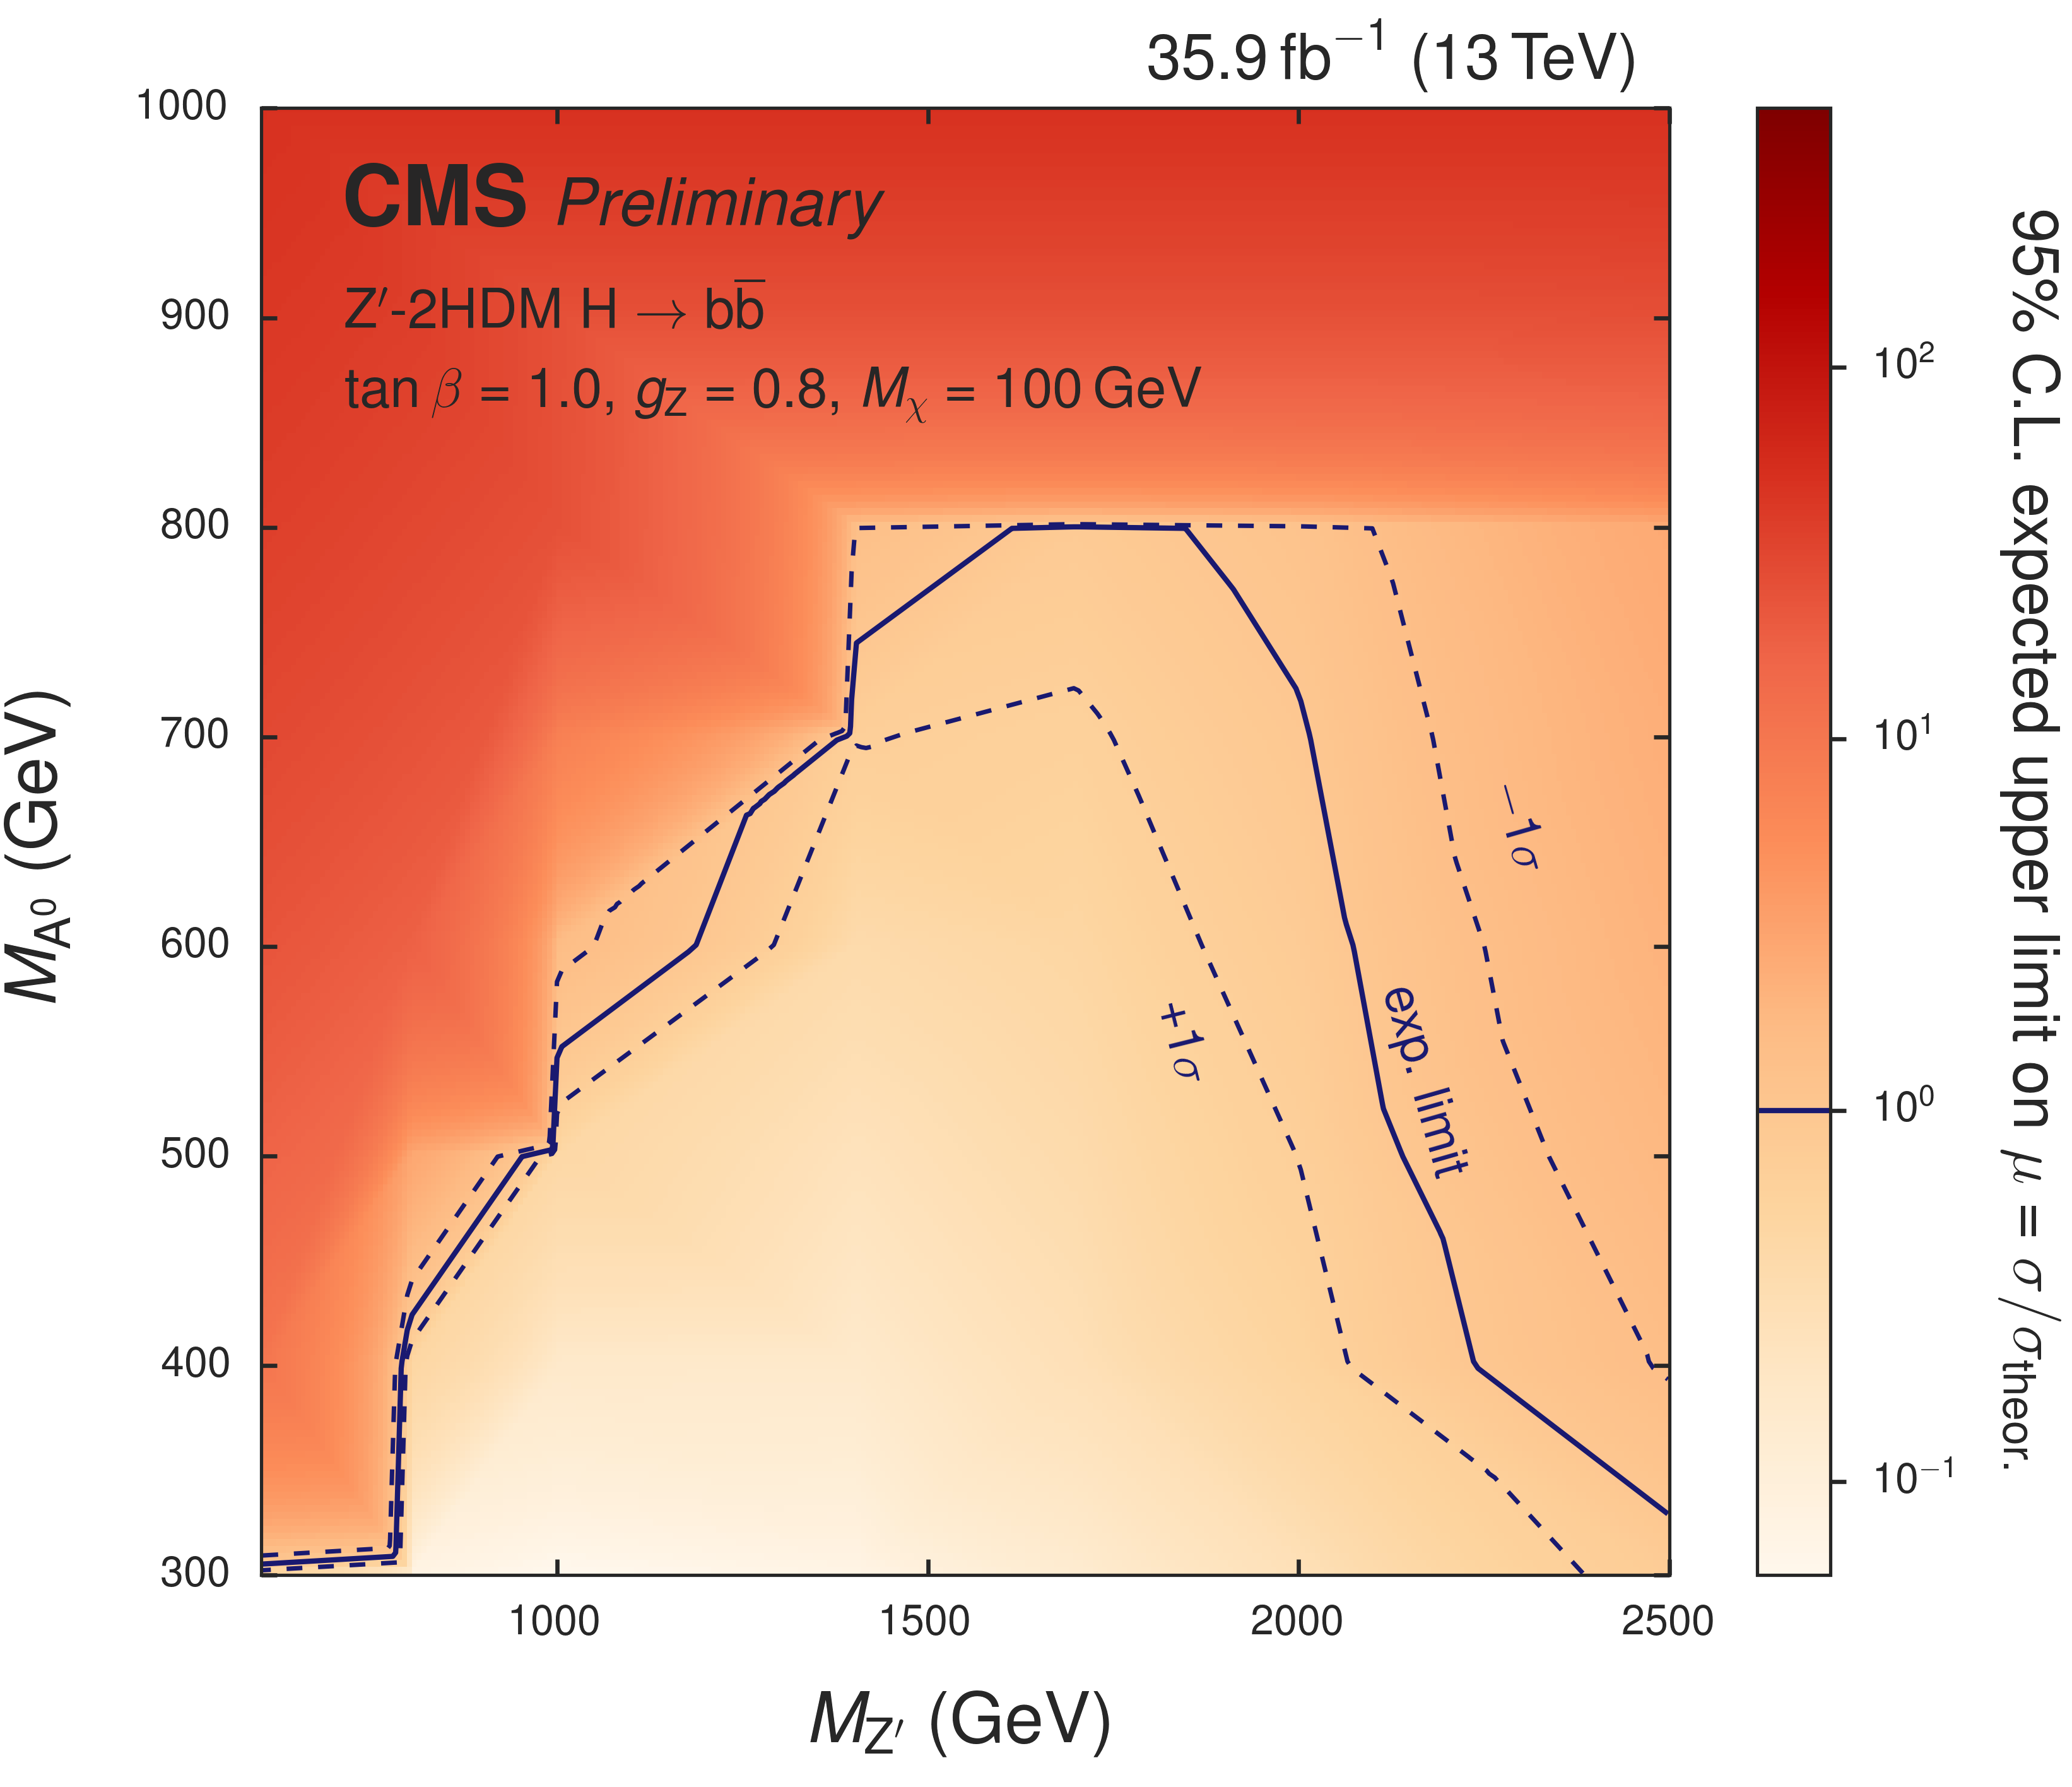
\includegraphics[width=0.475\textwidth]{limits_2hdm2d.png}
   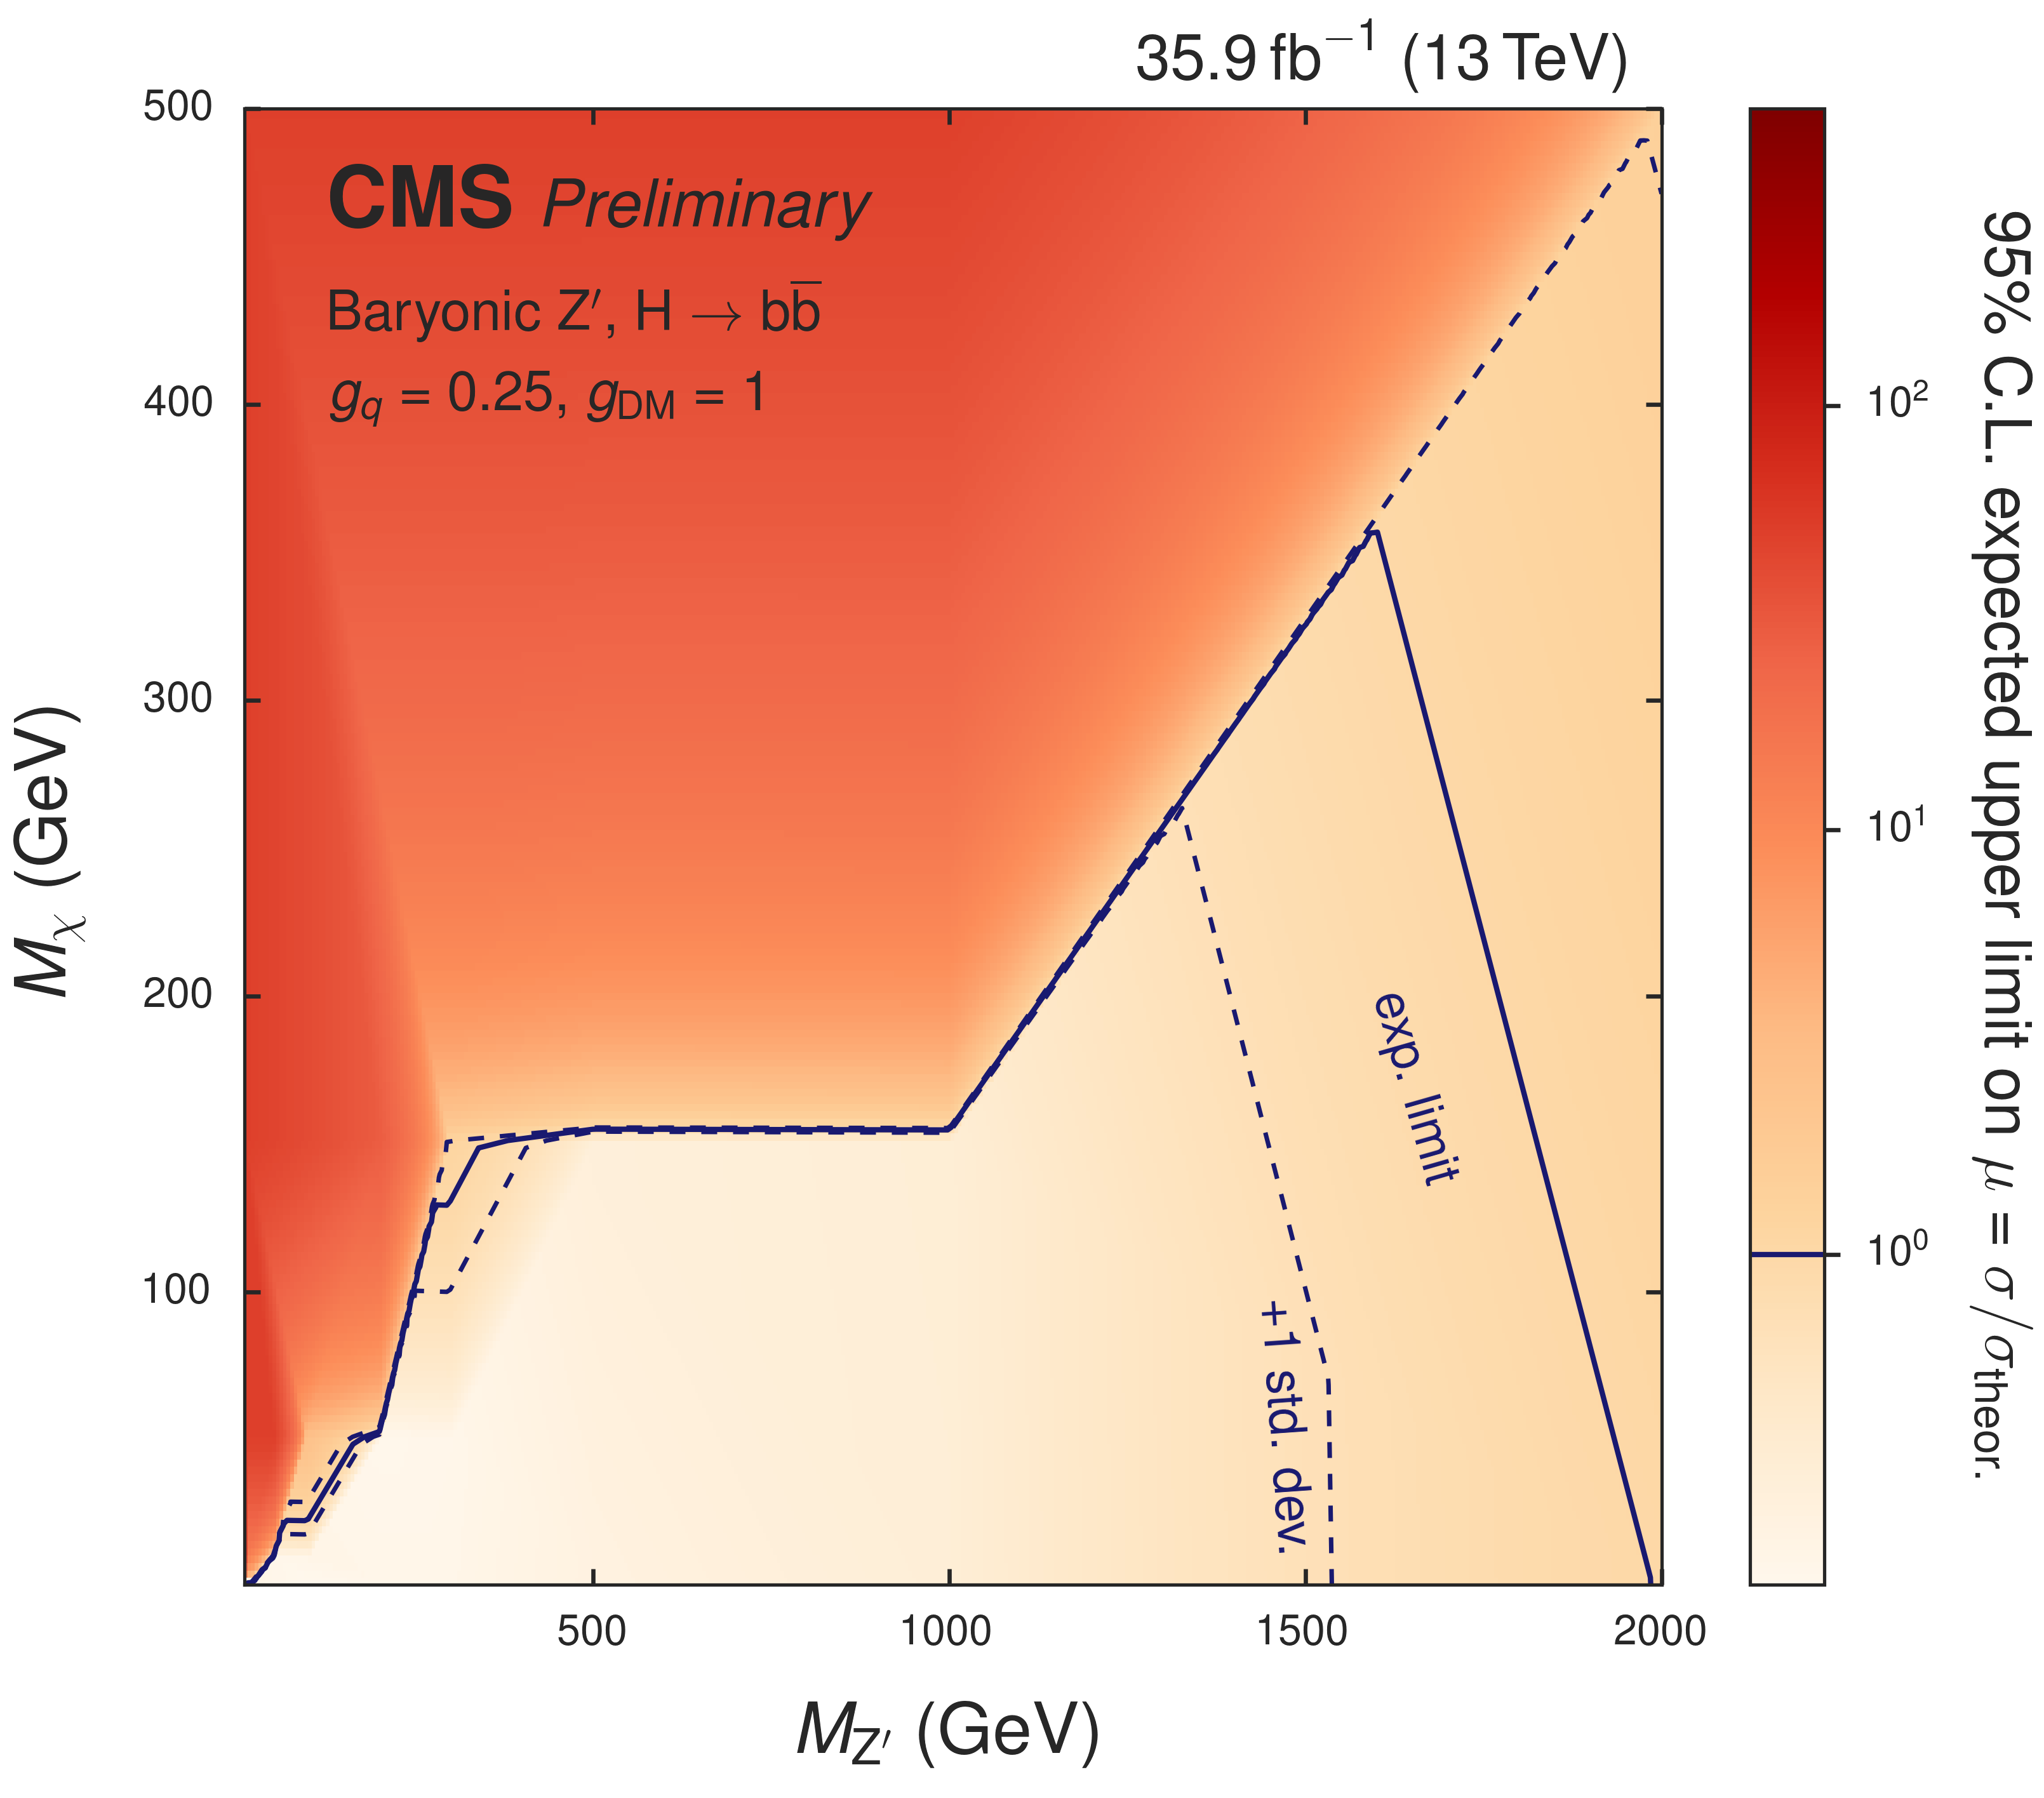
\includegraphics[width=0.475\textwidth]{limits_barzp2d.png}
   \caption{Left: limits on the signal strength for the Z'-2HDM model. Right: limits on the signal strength modified for the Baryonic 
Z' model. }
   \label{fig:limits}
\end{figure}


%%%%%%%%%%%%%%%%%%%%%%%%%%%%%%%%%%%%%%%%%%%%%%%%%%%%%%%%%%%%%%%%%%%%%%%%%%%%%%%%%%%%%%%%%%%%%%%%%%%%%%%%%%%%%%%%%%%%%%%%%%%%%%%%%%%%
\section{Searches for DM mediators via their visible decays}

Instead of looking for the production of DM particles in signatures with \ptvecmiss, we could also look directly for the mediators 
that mediate the DM-SM interaction via their visible decays. Since the production of mediators at LHC requires non-zero coupling of 
mediators to the SM quarks, all we need to do is to replace the decays of mediators into DM particles with the decays into a pair of 
SM quarks, as in Fig.~\ref{fig:transformation}. Given that the coupling of \Az to the SM particles is Yukawa-like, the \Az-top 
coupling is actually the largest. However, the decay topology would be more complex. Therefore, we decide to focus on the decays to 
a pair of b quarks and our final state consists of four b quarks. My undergraduate student Shu-Xiao Liu is working with me on this 
project. Initially we were focusing on the same 4-b final state but from the baryonic Z' model, see Fig.~\ref{fig:transb}. However, 
the ISR diagram (diagram 2 of Fig.~\ref{fig:transb}) is Yukawa-suppressed, the dominant production from diagram 1 does not always 
produce a resonant structure in the invariant mass spectrum of the \cPqb\cPaqb pair (from the \cPZpr decay); this poses a problem 
in our search and a narrow mass window selection cannot be applied. Therefore, we decide to focus on the Z'-2HDM model. 

In this case, we have a signature with $X\rightarrow Y_1 Y_2\rightarrow ZZZZ$. We had some discussion with Dr.~Maxime~Gouzevitch and 
Dr.~Devdatta~Majumder, with whom we worked together on the searches for resonances decaying to dihiggs final state. Maxime suggested 
us to try a technique discussed in JHEP 1307 (2013) 148. The basic idea is to apply similar kinematic selection in three different 
kinematic regimes: (i) both \Az and the Higgs boson are boosted, resulting in two AK8 jets, (ii) both \Az and the Higgs boson are 
non-boosted, resulting in four AK4 jets, (iii) Only one of the bosons is boosted, resulting in one AK8 jets and two AK4 jets.
The selection variables include the mass window, \pt asymmetry, $\Delta \eta$, and b-tagging. Shu-Xiao had produced 42 mass points 
of Z'-2HDM signals with various \maz and \mzp to cover these three kinematic regimes. He would first compare the distributions of 
signals and background to optimize his selection and find the criteria that makes the signal efficiency flat. The next thing he would 
try is to employ alphabet-assisted bump hunt to estimate the background.

\begin{figure}[htbp]
   \centering
   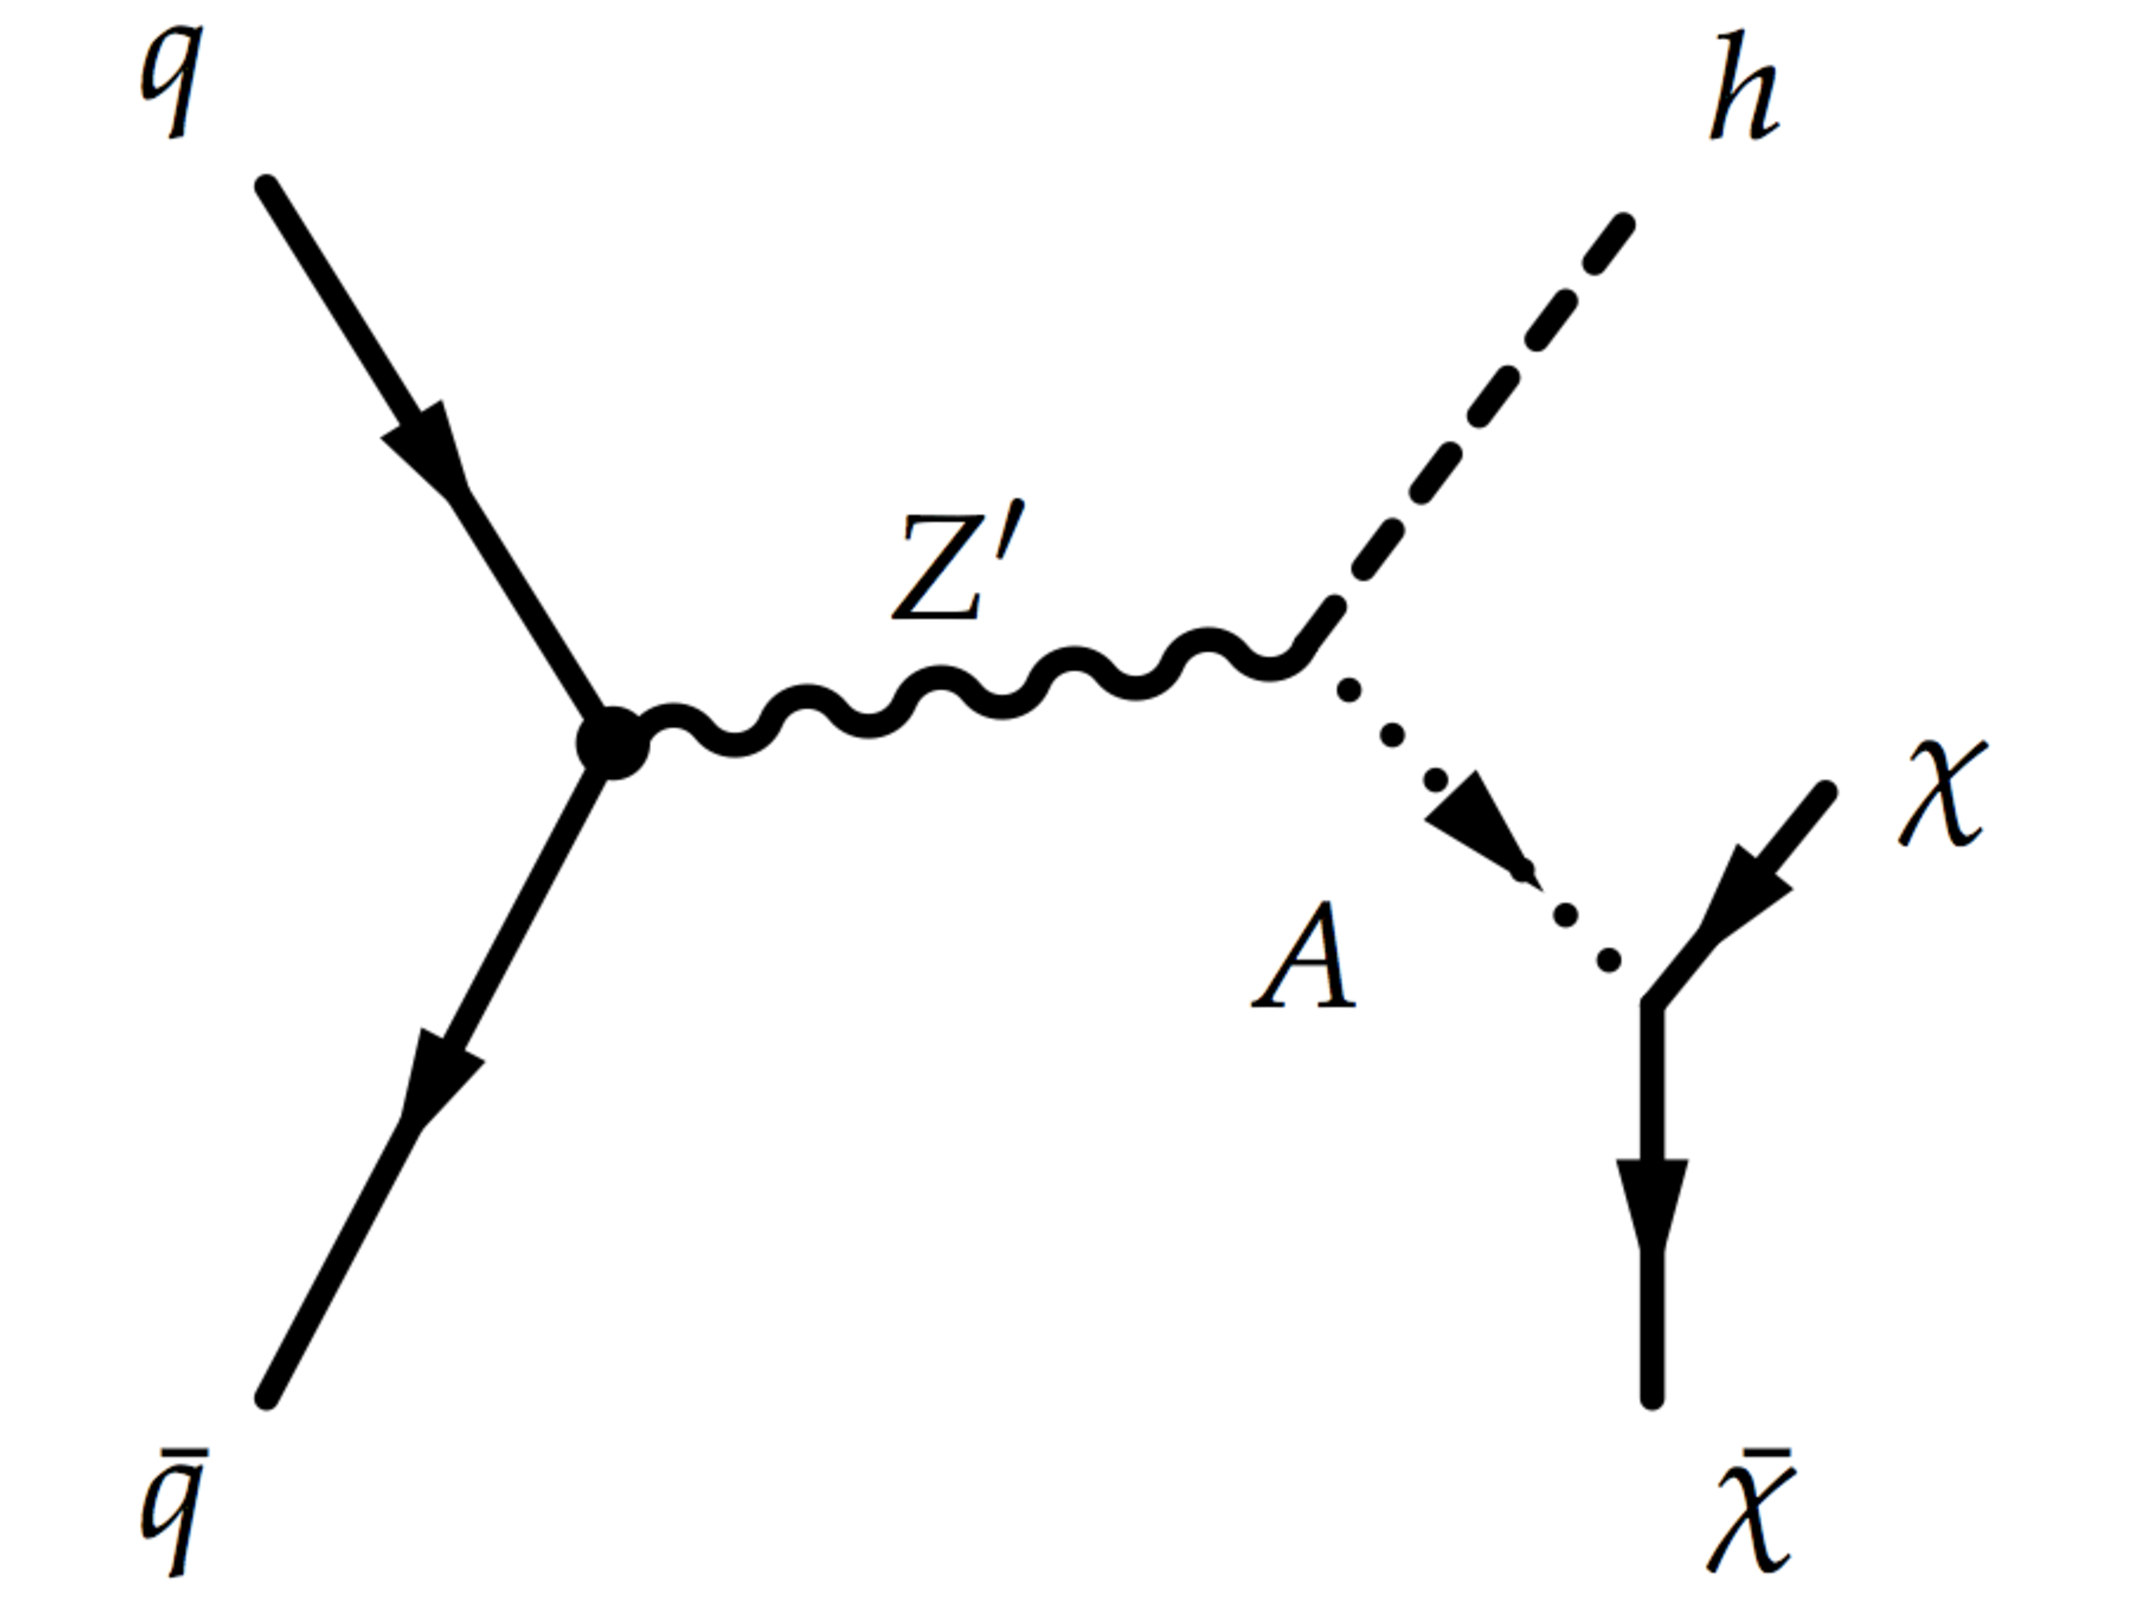
\includegraphics[width=0.475\textwidth]{Figure_001.pdf}
   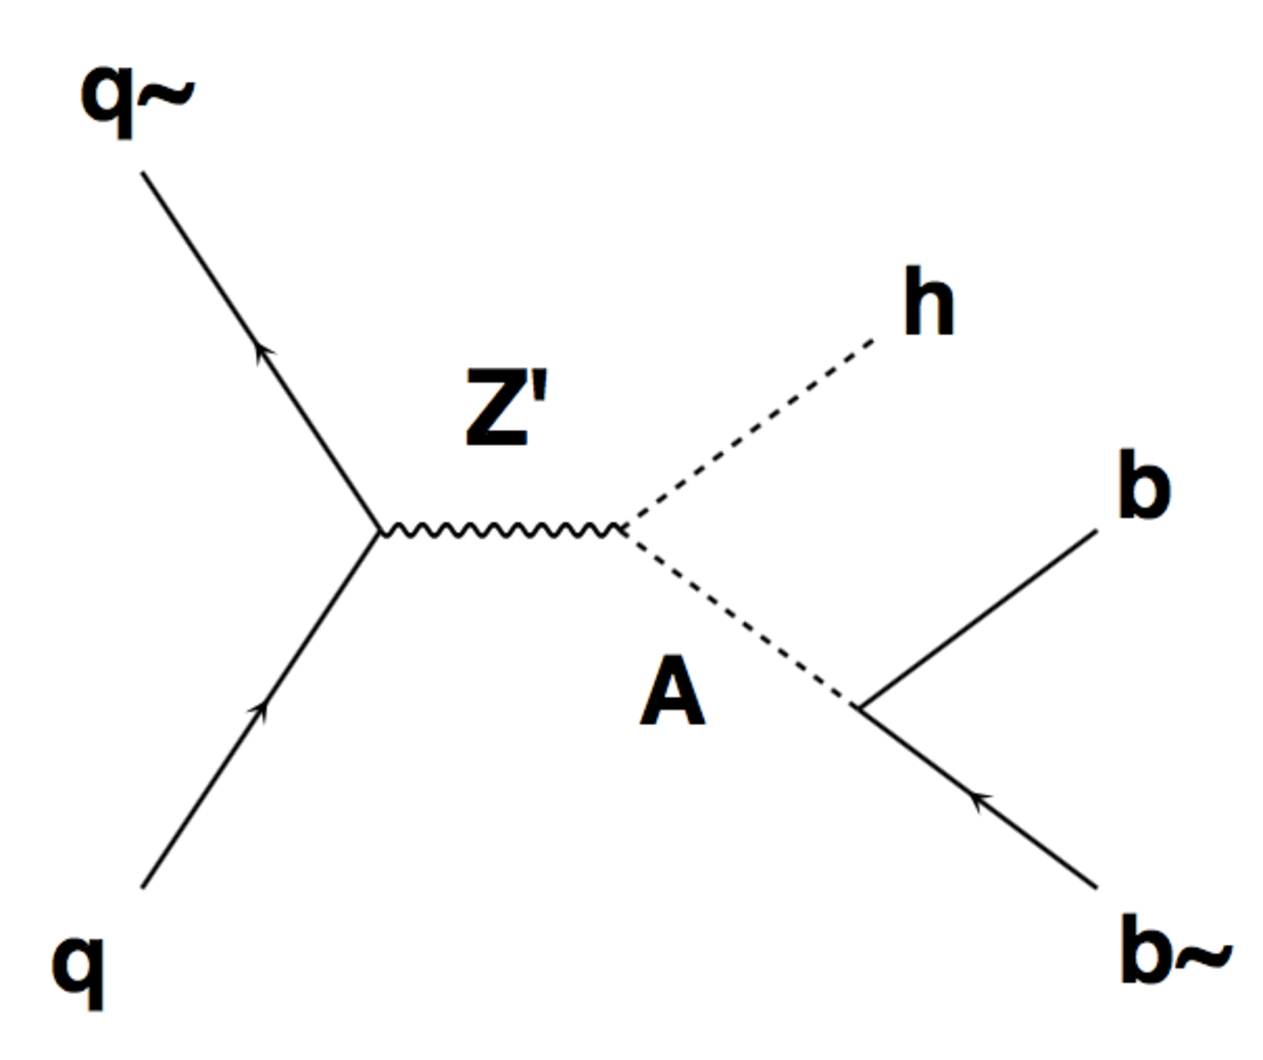
\includegraphics[width=0.475\textwidth]{Figure_001_modified.pdf}
   \caption{Left: Leading order Feynman diagram of the \cPZpr-2HDM ``simplified model''. A pseudoscalar boson \Az decaying into 
invisible dark matter is produced from the decay of an on-shell $\cPZpr$ resonance. This gives rise to a Higgs boson and missing transverse momentum. Right: a similar physics process with the \Az decaying into a pair of SM b quarks, \cPqb\cPaqb.}
   \label{fig:transformation}
\end{figure}

\begin{figure}[htbp]
   \centering
   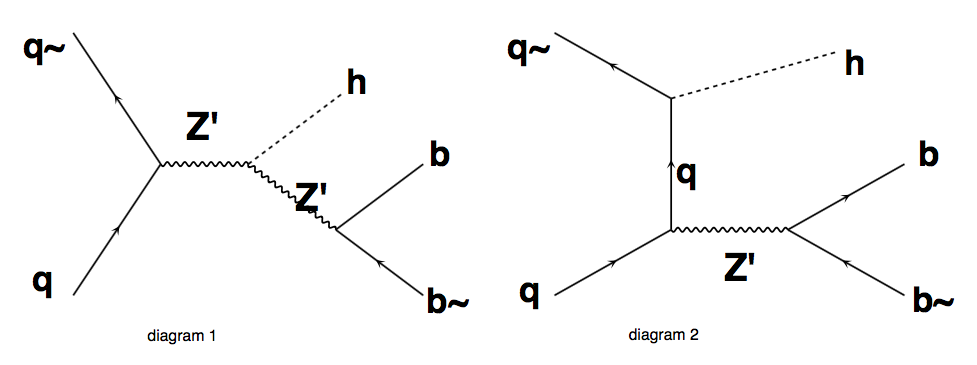
\includegraphics[width=0.8\textwidth]{baryonicZ.png}
   \caption{Leading order Feynman diagram of the baryonic-Z' ``simplified model''. In diagram 1 (left), the \cPZpr 
radiates a Higgs boson and further decays into a pair of DM particles; while in diagram 2 (right), the Higgs boson is 
produced from the initial state radiation of the incoming quarks.}
   \label{fig:transb}
\end{figure}


%%%%%%%%%%%%%%%%%%%%%%%%%%%%%%%%%%%%%%%%%%%%%%%%%%%%%%%%
\section{Analysis of the July 2017 HGC test beam data}

Due to my trip to the EPS 2017, I could not participate in taking shifts for the HGC test beam. However, my Ph.D. student 
Yu-Hsiang~Chang and undergraduate student Shu-Xiao Liu had taken shifts for the May and July 2017 HGC test beam. 
Yu-Hsiang also worked with an NTU master student Chia-Hung Chien on the estimation of pedestals, while I started working 
with the IHEP postdoc Francesco Romeo and Ph.D. student Binghuan Li on the calibration of minimum ionizing particles 
(MIPs). Unlike the test beam data last year and the old skiroc, the new skiroc CMS and the July muon beam data are 
noisier. A master student from Achen, Thorben Quast, proposed to use the data from wire chambers to select clean MIP 
events, see Fig.~\ref{fig:DWC} for the relative position of each wire chamber. Unfortunately, during the HGC data taking, 
only wire chamber E was connected to high voltage and functional. Therefore, what Thorben did was to correlate the 
trigger counts in the wire chamber data with those of the HGC data and then study only the events concentrated in the 
expected $x$ and $y$ positions of wire chamber. He passed the histograms of only one skiroc to Francesco and myself. 

I tried to fit the distributions of ADC counts from skiroc 28 and channel 22 first with a simple $\chi^2$ fit, 
without using RooFit. I fitted the noise to a Breit-Wigner function and the signal to a ECAL-pulse shape function or 
Landau function (see Fig.~\ref{fig:normalfit}). Later, I got myself familar with RooFit and fitted the 
noise with a Gaussian and the signal a Landau convoluted with a Gaussian (see Fig.~\ref{fig:roofit}). 
The peak value that indicates the MIP signal ranges from 35 ADC counts to 38 ADC counts, depending on the function of 
signal shapes. 


\begin{figure}[htbp]
   \centering
   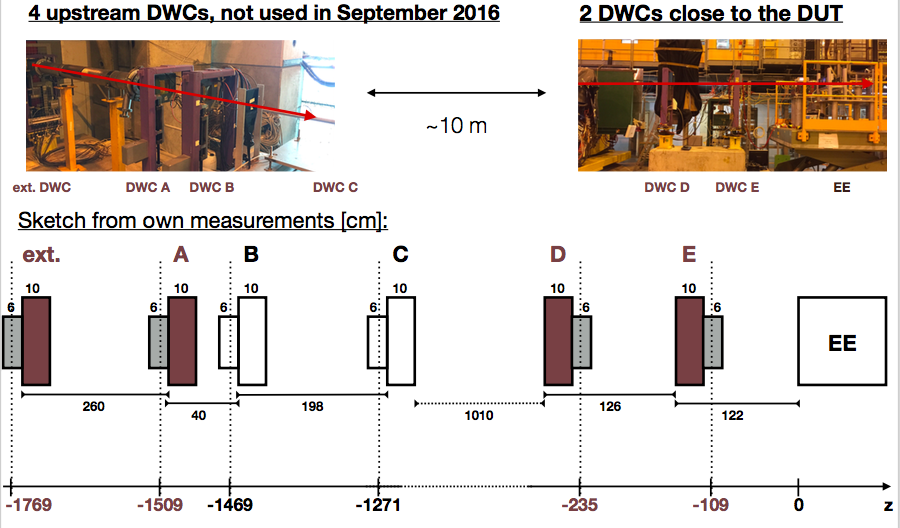
\includegraphics[width=0.8\textwidth]{DWC.png}
   \caption{The relative position of the wire chambers at the CERN H2 test beam area, produced by Thorben Quast.}
   \label{fig:DWC}
\end{figure}

\begin{figure}[htbp]
   \centering
   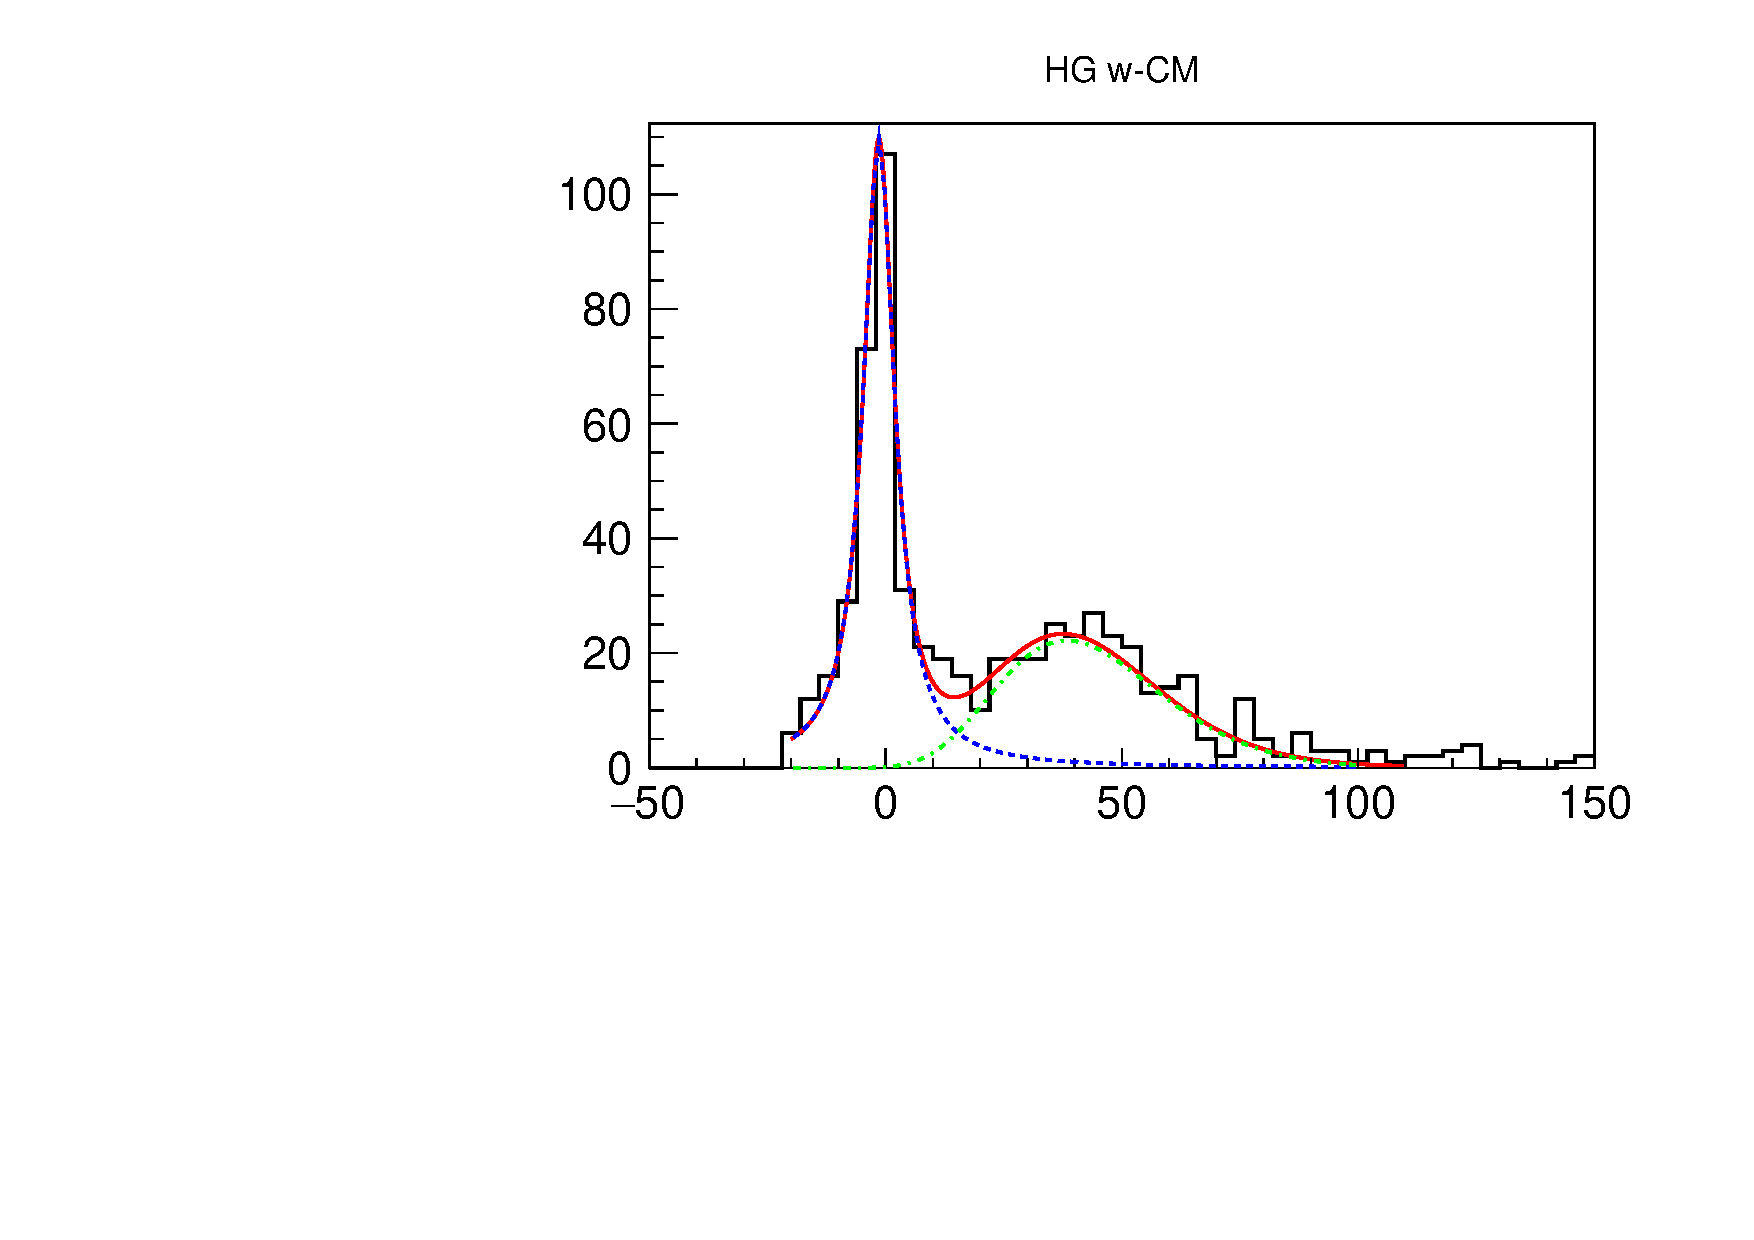
\includegraphics[width=0.45\textwidth]{trial_fitpulse_skiroc28_chan22.pdf}
   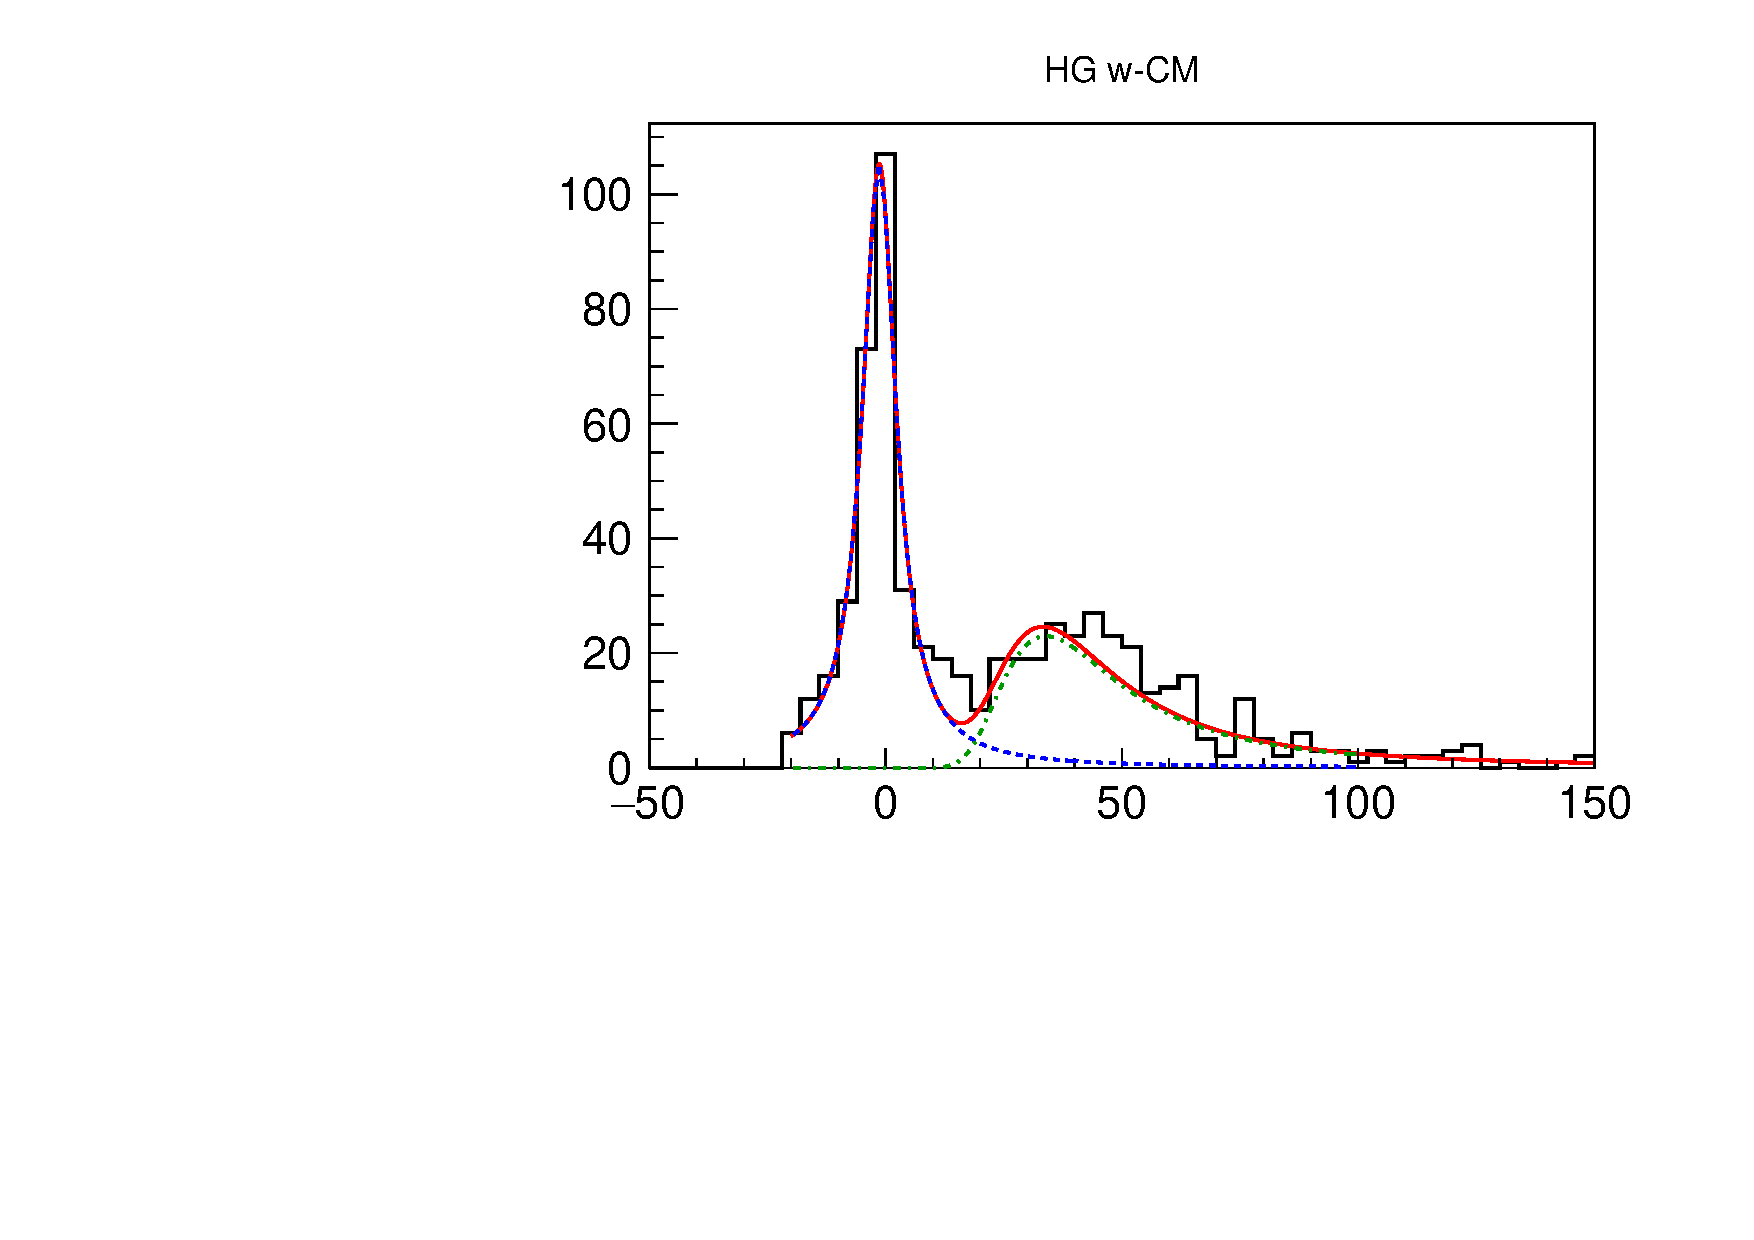
\includegraphics[width=0.45\textwidth]{trial_fitlandau_skiroc28_chan22.pdf}
   \caption{The results of $\chi^2$ fit to the distribution of ADC counts from skiroc 28 channel 22, 
 after making selection based on wire chamber data. The noise near zero is fitted with a Breit-Wigner function 
 while the MIP signal is fitted with a ECAL-pulse shape (left) or a Landau function (right). The MIP peak 
 occurs at 38.4$\pm$2.2 ADC counts when using the ECAL-pulse shape and 35.7$\pm$1.5 ADC counts when using a 
 Landau function.}
   \label{fig:normalfit}
\end{figure}

\begin{figure}[htbp]
   \centering
   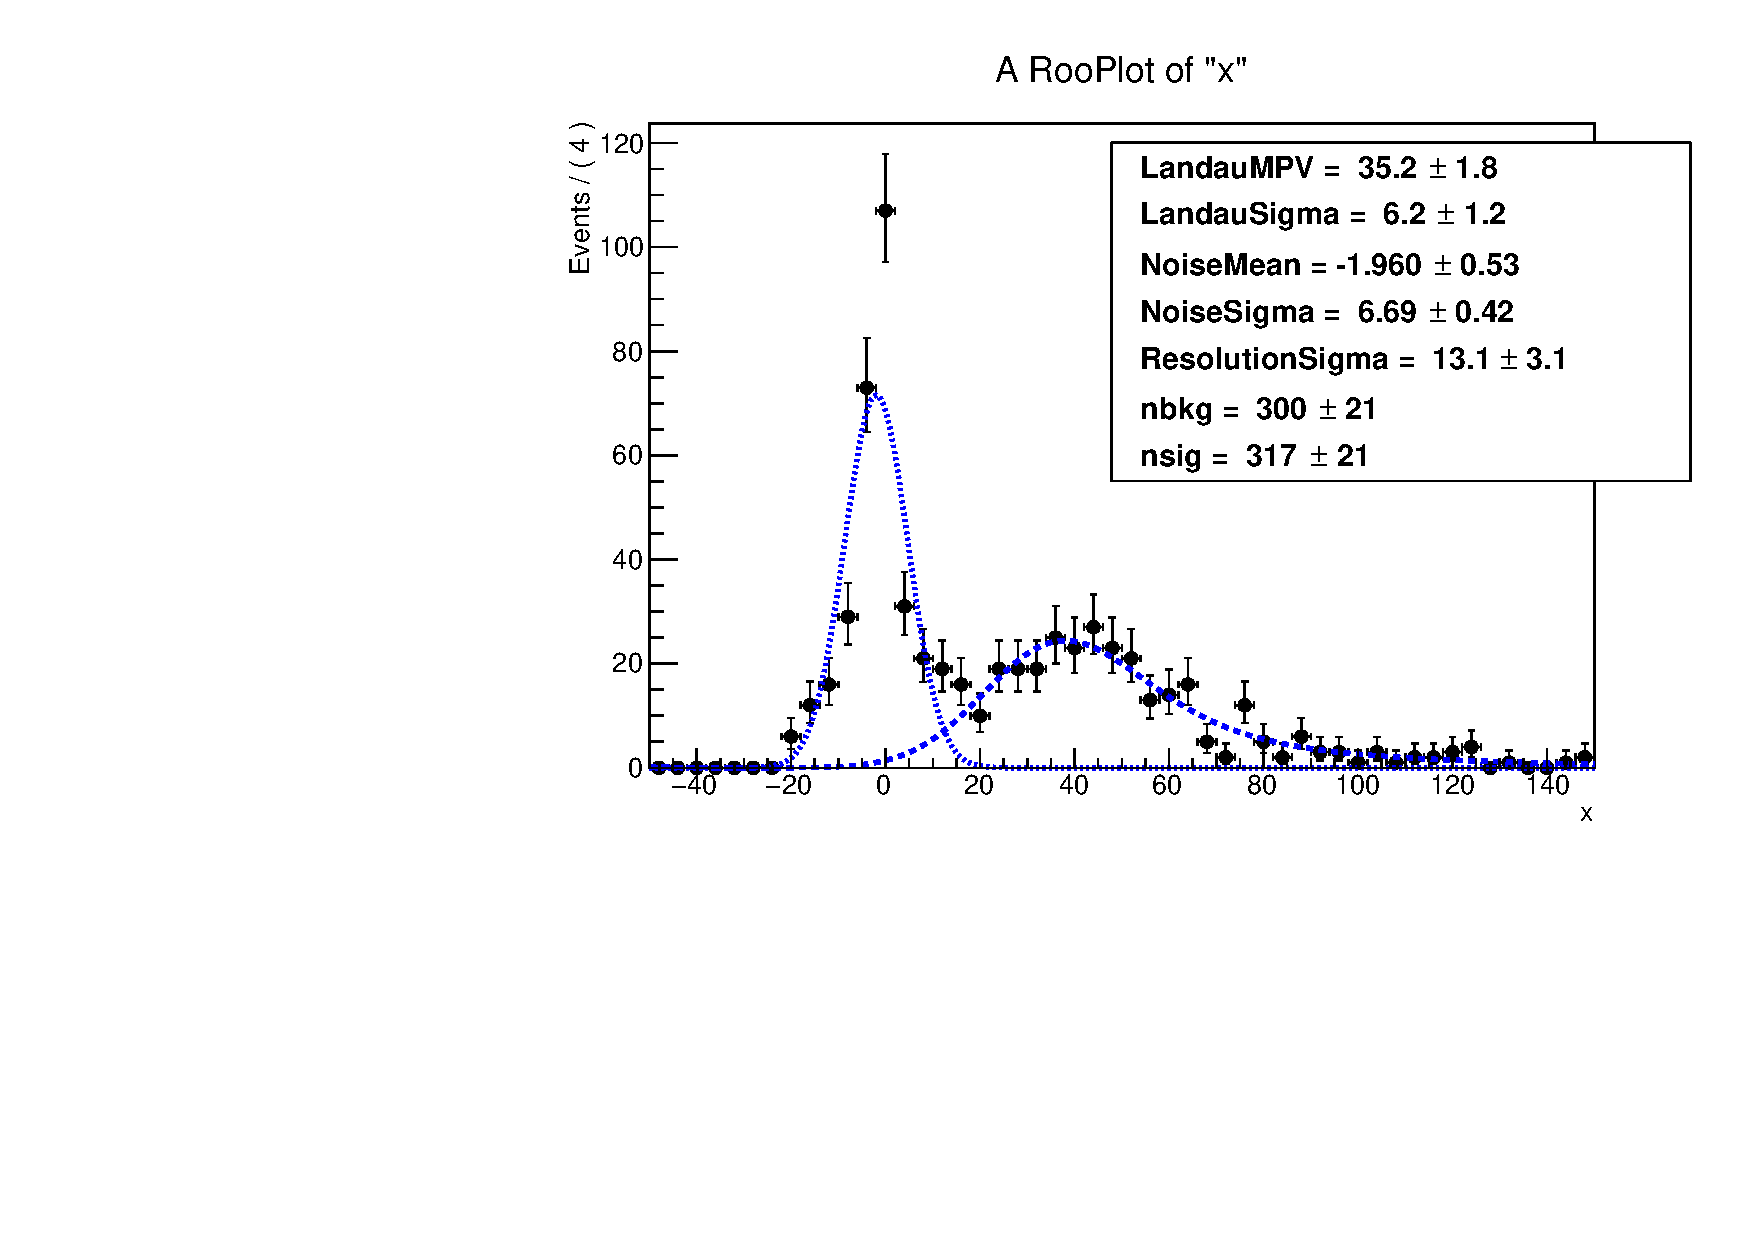
\includegraphics[width=0.8\textwidth]{roofit_skiroc28_chan22.pdf}
   \caption{The results of binned likelihood fit with RooFit to the distribution of ADC counts from skiroc 28 channel 22, 
 after making selection based on wire chamber data. The noise near zero is fitted with a Gaussian function 
 while the MIP signal is fitted with a Landau convoluted with a Gaussian. The MIP peak 
 occurs at 35.2$\pm$1.8 ADC counts.}
   \label{fig:roofit}
\end{figure}


%%%%%%%%%%%%%%%%%%%%%%%%%%%%%%%%%%%%%%%%%%%%%%%%%%%%%%%%
\section{Implementing the analysis ntuple framework and prepare for 2017 data taking}
 While finishing up the 2016 data analysis, we also have to modify our own 
analysis code to accommodate the new CMS software framework in 2017. We are 
moving from CMSSW\_8\_0\_X to CMSSW\_9\_2\_X. In addition, the AK8 CHS jets 
are not supported any more and by default miniAOD only saves AK8 Puppi jets. I 
also added code for the new jet substructure variable $N_2$ and double b-tagger 
for CA15 jets. We are planning to synchronize our ntuples with the MIT 
framework as soon as we are done with the 2016 analysis approval 
procedures. The codes for the 2017 data are now at Ref.~\cite{EikoCode}.

\section{Testing and preparing the code to compute jet substructure variables 
using calo hits for the 100-TeV collider}

During May and June 2017, I have started to check the jet substructure variables for the 100-TeV collider. I started by 
producing distributions of variables including $\tau_{21}$, various energy correlation functions (ECFs) c2\_b1, d2\_b1, 
n2\_b1, trimmed mass, etc, by reconstructing these variables with calorimeter clusters. I compared two physics processes 
$\cPZpr\rightarrow \cPq\cPaq$ (background-like) and $\cPZpr\rightarrow$WW (signal-like). 
However, when the Z' mass is as large as 40~\TeV, I did not see improvement of separation when reducing the hadron 
calorimeter cell size from 20~cm to 5~cm to 1~cm~\cite{Eikojsubcluster}. The separation is quantified by computing the 
area of overlapped region from the normalized signal and background distributions. 
Prof.~Ashutosh~Kotwal from Duke University 
suggested me to use ECAL and HCAL hits as input instead of calorimeter clusters. However, if I did not apply any 
selections to remove low-energy ECAL/HCAL hits, it took forever to process one event, particularly for higher Z' mass.
 Therefore, I started by setting the minimum energy threshold of ECAL and HCAL hits to 0.5~\GeV; this selection reduced 
the number of hits down by a factor of ten. I tried the new code for the default hadron calorimeter cell size 
5~cm$\times$5~cm and the separation did improve (see Fig.~\ref{fig:calohit}). I passed the code to my undergraduate 
student Chih-Hsiang Yeh so that he could run for all energies and all detector configurations.

\begin{figure}[htbp]
   \centering
   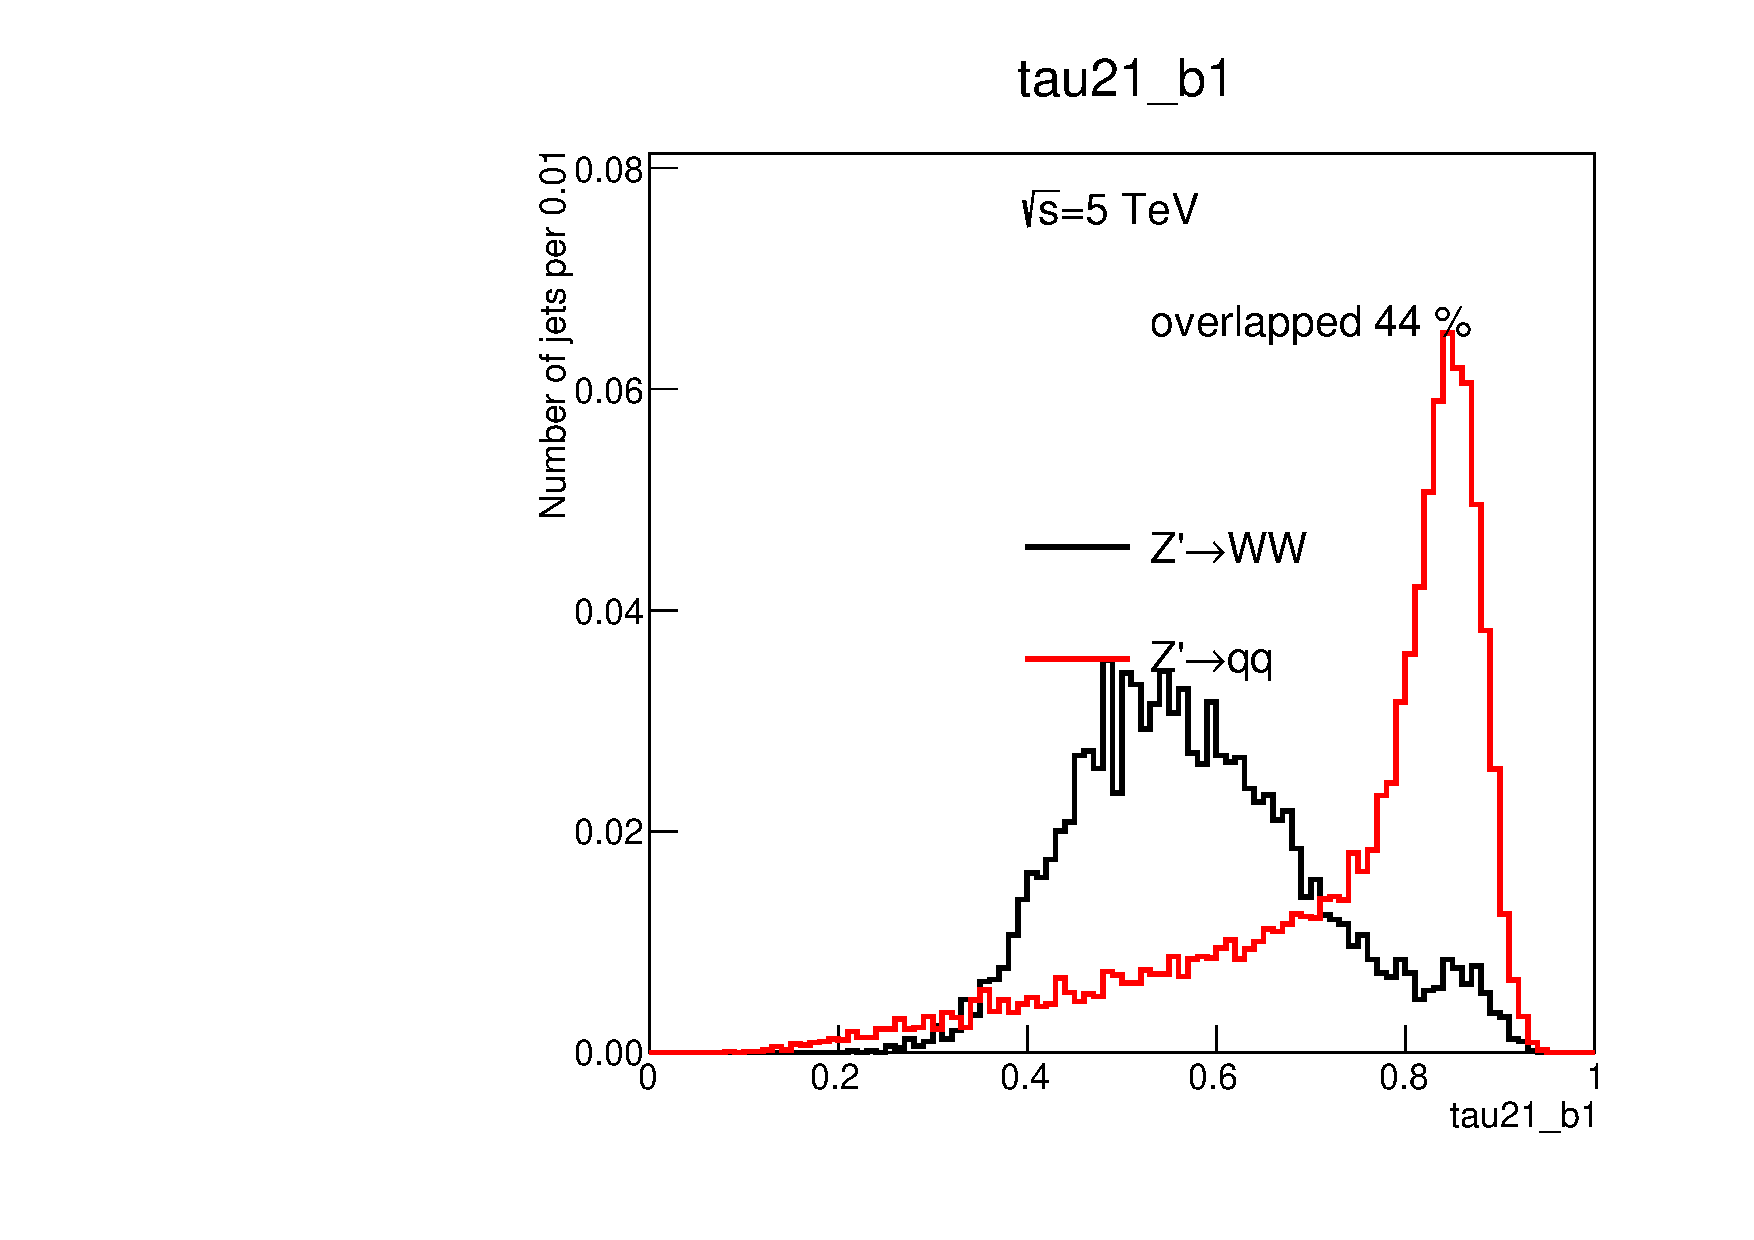
\includegraphics[width=0.475\textwidth]{tau21.pdf}
   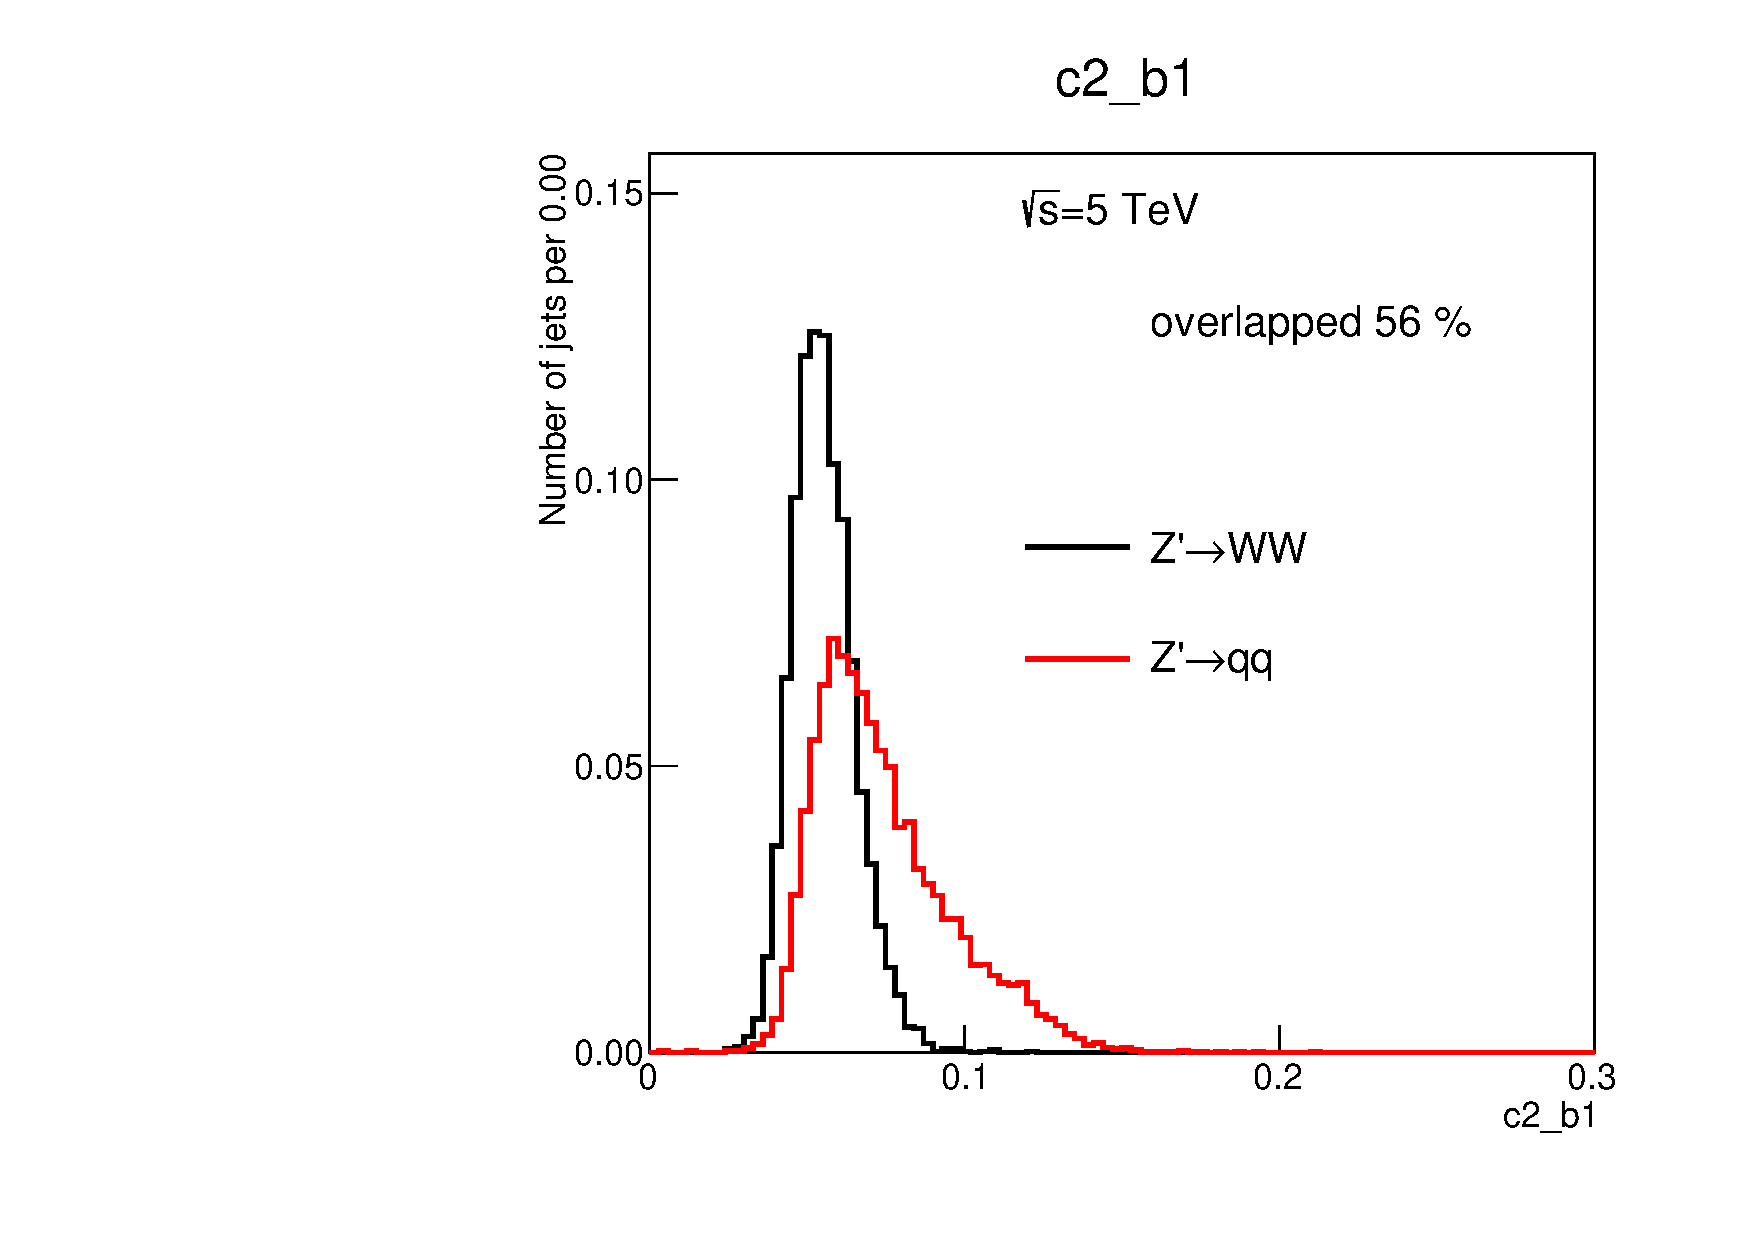
\includegraphics[width=0.475\textwidth]{c2_b1.pdf}
   \caption{The $\tau_{21}$ (left) and c2\_b1 (right) variables built with ECAL/HCAL hits from the $\cPZpr\rightarrow \cPq\cPaq$ (background-like) and $\cPZpr\rightarrow$WW (signal-like) events. The mass of the \cPZpr\ is set to 5~\TeV.}
   \label{fig:calohit}
\end{figure}










\bibliography{auto_generated}

